\chapter{Ionización de átomos y moléculas: el método de inversión depurada}
\label{chap:iondim}

%%%%%%%%%%%%%%%%%%%%%%%%%%%%%%%%%%%%%%%%%%%%%%%%%%%%%%%%%%%%%%%%%%%%%%%%
\section{Introducción}
%%%%%%%%%%%%%%%%%%%%%%%%%%%%%%%%%%%%%%%%%%%%%%%%%%%%%%%%%%%%%%%%%%%%%%%%

Las probabilidades de transición en una colisión inelástica se pueden 
obtener a partir de la correcta representación de los estados inicial y 
final del blanco. En general, la resolución de las ecuaciones de 
Schr\"odinger de sistemas multielectrónicos atómicos implementa el 
modelo de partículas independientes en conjunción con la aproximación 
de campo central~\cite{Bransden:03,Cowan:81}. La descripción de la 
estructura electrónica de sistemas moleculares constituye un desafío 
desde el punto de vista teórico debido a su geometría multicéntrica. Sin 
embargo, se han propuesto diversas aproximaciones para tal 
fin~\cite{Helgaker:00,Schaefer:04}. 
En el marco de la teoría cuántica, los procesos colisionales de átomos 
y moléculas simples debido al impacto de diversos proyectiles se ha 
estudiado de forma extensa. A grandes rasgos, los métodos desarrollados
para predecirlos se puden clasificar en dos grupos: las aproximaciones 
perturbativas, entre las que se destacan las de Born~\cite{Bates:62,
McDowell:61} y de onda distorcionada~\cite{Crothers:10,Rivarola:87}, y 
el grupo de métodos no perturbativos, con técnicas tales como los de 
acoplamiento cercano~\cite{Pindzola:07,Burke:11,Bray:17,Zatsarinny:04,
McCurdy:04}. 

En general, los procesos colisionales simples se basan en la 
aproximación de electrón activo. En la ionización, el electrón activo 
está inicialmente ligado y luego de la colisión se encuentra libre. La 
descripción de los estados ligados es relativamente simple mientras que 
la representación de los continuos presenta cierta dificultad. Así, es 
conveniente contar con un potencial efectivo local que permita obtener 
de forma directa las funciones de onda de las partículas interactuantes. 
Se han desarrollado diversas metodologías para el diseño de potenciales 
efectivos en blancos atómicos~\cite{Hibbert:82,Gombas:56,Green:69,
Klapisch:71,Phillips:59,Herman:63,Dalgarno:70,Bayliss:77,Cowan:76,
Lee:77} y moleculares~\cite{Menchero:10,Granados:16}. Una técnica 
conocida es el método de inversión, que consiste en determinar 
potenciales centrales a partir de funciones de onda y/o densidades 
electrónicas. Este procedimiento se ha estudiado de forma extensa en la 
teoría del funcional de la densidad~(\acs{dft}, por sus siglas en 
inglés), en donde se emplean densidades del estado 
fundamental~\cite{Wu:03,Gaiduk:13,Ryabinkin:15,Schipper:97,deSilva:12,
Kananenka:13,Jacob:11}. En la teoría de colisiones atómicas, el método 
de inversión fue sugerido por Hilton~\textit{et al.} en aplicaciones 
circunscriptas al cálculo de procesos de fotoionización~\cite{Hilton:77,
Suzer:77,Hilton:79,Hilton:80,Crljen:87}. A su vez, estos estudios se 
refieren a investigaciones previas en polarizabilidad 
atómica~\cite{Sternheimer:54,Dalgarno:59}. Sin embargo, estos trabajos 
se enfocan en los resultados de secciones eficaces de fotoionización y 
no presentan detalles acerca de la calidad de los potenciales y las 
funciones de onda resultantes. 

En este Capítulo se estudia la estructura de átomos y moléculas pequeñas
en procesos colisionales simples. La descripción de los blancos se 
obtiene de potenciales que resultan de la implementación del método de 
inversión depurada~(\acs{dim}). El desarrollo teórico de esta técnica se 
presenta en la Sección~\ref{sec:dimatomos}. El DIM consiste en la 
inversión de ecuaciones de un electrón, cuyas soluciones se conocen. 
Luego, los potenciales resultantes se ajustan mediante expresiones 
analíticas con las condiciones de borde apropiadas y se optimizan 
variando los parámetros que los definen. El método de inversión depurada 
es general y se puede aplicar a soluciones que se obtienen en el marco 
de diversas aproximaciones. Con el fin de ilustrar su aplicación en 
átomos y moléculas, las soluciones que se implementan en este trabajo 
están dadas por la teoría de Hartree--Fock~(\acs{hf}). La implementación 
del DIM a partir de orbitales HF se presenta en la 
Sección~\ref{subsec:invHF}. Si bien el procedimiento de inversión es 
directo, los potenciales resultantes presentan polos y divergencias. 
El origen de estos defectos se discuten al final de este Capítulo, en la 
Sección~\ref{sec:discusionHF}. Como corolario de la implementación del 
DIM en orbitales HF, y asumiendo la validez de la separación de los 
términos de intercambio y correlación, en la 
Sección~\ref{sec:corolarios} se presentan potenciales de intercambio 
orbitales ``exactos''. A partir de los potenciales DIM también se pueden 
calcular las energías totales y de intercambio de forma directa. En la 
Sección~\ref{sec:dimmoleculas}, el DIM se extiende para describir 
moléculas simples. A diferencia del caso atómico, los orbitales 
moleculares se expresan a partir de conjuntos de base de orbitales tipo 
Gaussianos, de manera que el método de inversión depurada requiere 
algunas modificaciones.

El objetivo principal de este Capítulo es ilustrar el uso efectivo de 
potenciales DIM en la teoría de colisiones atómicas. Para este fin 
se realizan ciertas simplificaciones: los cálculos están restringidos a 
los Hamiltonianos que describen el proyectil, el blanco y el electrón 
activo, y los elementos de la matriz de transición se consideran en 
primer orden perturbativo. %Se examinará la ionización de atómos multielectrónicos y moléculas con pocos átomos debido al impacto de protones y fotones. 
Así, el marco teórico de los procesos colisionales estará dado por la 
primera aproximación de Born (FBA, ver Apéndice~\ref{app:born}), que 
reproduce razonablemente las secciones eficaces experimentales de 
diversos procesos en el rango intermedio--alto de energías incidentes 
del proyectil. Dentro de este rango de energía y orden de aproximación, 
los orbitales de Hartree--Fock proporcionan una buena descripción de las 
secciones eficaces del blanco en el límite de altas energías.

Los resultados de la implementación del método de inversión depurada 
para describir la estructura de blancos atómicos y moleculares se 
presentan en la Sección~\ref{subsec:dimtarget}. La efectividad del DIM 
se evalúa a partir de su habilidad para describir la estructura 
electrónica del blanco y predecir el proceso colisional al que son 
sometidos. Las predicciones resultantes de la combinación de los 
potenciales DIM y la FBA para describir la ionización simple de átomos y 
moléculas por impacto de protones y fotones se muestra en la 
Sección~\ref{subsec:procol}. En total, se presentan 
resultados de cuatro blancos: helio, nitrógeno, neón y metano. Sin 
embargo, una gran cantidad de potenciales DIM se han presentado en 
diversas publicaciones en los últimos años~\cite{Mendez:16,Mendez:19dim,
Mendez:18}. Además, actualmente se está trabajando en una base de datos 
de estructura de átomos y potenciales que cubre todos los elementos no 
relativistas de la tabla periodica, que será de libre acceso. 
Las conclusiones de este trabajo se encuentran en la 
Sección~\ref{sec:conclu-dim}.

%%%%%%%%%%%%%%%%%%%%%%%%%%%%%%%%%%%%%%%%%%%%%%%%%%%%%%%%%%%%%%%%%%%%%%%%
\section{Método de la inversión depurada (DIM)}
%%%%%%%%%%%%%%%%%%%%%%%%%%%%%%%%%%%%%%%%%%%%%%%%%%%%%%%%%%%%%%%%%%%%%%%%
\label{sec:dimatomos}

El método de inversión depurada consiste en resolver el problema inverso
dado por la ecuación de Schr\"odinger de un sistema de $N$ electrones y 
carga $Z$ en la aproximación de campo central, 
\begin{equation}
 \left[ -\frac{1}{2}\frac{d^2}{dr^2} + \frac{l(l+1)}{2r^2} +
 V(r) \right] u_{nl}(r) = \varepsilon_{nl} \, u_{nl}(r)\,,
\label{eq:eqSchroRadial}
\end{equation}
donde $V(r)$ es el potencial que gobierna la dinámica del átomo, 
$u_{nl}$ es la función radial reducida y $\varepsilon_{nl}$ la energía
del orbital $nl$. Si las soluciones de la Ec.~(\ref{eq:eqSchroRadial}) 
se conocen, es posible definir un \textit{potencial invertido} que las 
genera
\begin{equation}
V_{nl}(r) = 
\frac{1}{2}\frac{1}{u_{nl}(r)} \frac{d^2\,u_{nl}(r)}{dr^{2}} - 
\frac{l(l+1)}{2r^{2}}+\varepsilon_{nl} \,.
\label{eq:Vinv}
\end{equation}

Suponiendo que el potencial invertido tienen una forma Coulombiana, 
ilustrado en la Fig.~\ref{fig:potycharge}(a), es conveniente definir una 
\textit{carga invertida} tal que
\begin{equation}
Z_{nl}(r) \equiv -r \, V_{nl}(r) \,.
\label{eq:Zinv}
\end{equation}
Esta carga efectiva, esquematizada en la Fig.~\ref{fig:potycharge}(b), 
deberá ser suave y cumplir con condiciones de borde definidos por la 
naturaleza del blanco a describir: en el origen la carga debe 
ser igual a la carga nuclear del átomo y asintóticamente, debido al 
apantallamiento electrónico, ésta es igual a uno. Esto es,
\begin{equation}
Z_{nl}(r) \, \rightarrow 
\bigg\{ 
\begin{array}{ll}
Z  \ \  & \ \ \text{:\ \ }r  \rightarrow 0 \,, \\ 
1           & \ \ \text{:\ \ }r  \rightarrow \infty \,.
\end{array}
\label{eq:Zasympt}
\end{equation} 
Luego, la carga invertida se ajusta con una expresión analítica que 
cumple con estas condiciones de borde.

\begin{figure}[t]
\centering
\includegraphics[width=0.93\textwidth]{dim/pot-charge.eps}
\caption[Características físicas del potencial y carga efectiva.]
{Ilustración de las características físicas esperadas del (a) potencial 
y (b) carga efectiva para el átomo de carga nuclear $Z$.}
\label{fig:potycharge}
\end{figure}

Debido a la presencia de la función de onda en 
el denominador de la Ec.~(\ref{eq:Vinv}), es posible que las cargas 
invertidas presenten defectos numéricos. De ser así, se restringe la 
región de ajuste descartando comportamientos inconsistentes con la 
naturaleza del blanco. En átomos, la carga DIM está dada por
\begin{equation}
Z_{nl}^{\mathrm{DIM}}(r)= \sum_{j=1}^{n} z_j e^{-\alpha_j r}+1 \,,
\label{eq:atomzDIM}
\end{equation}
donde $\Sigma_j z_j=Z-1$. Los parámetros $\left\{z_j,\alpha_j\right\}$ 
definen un potencial de prueba que se optimiza hasta reproducir las 
soluciones iniciales $u_{nl}$ y $\varepsilon_{nl}$ de manera precisa. 
%Para esto se minimiza una función de costo que se define a continuación.

La mayoría de los métodos de funcional de la densidad están basados en 
un principio variacional que minimiza el funcional de energía. Sin 
descartar su importancia, la energía es solo uno de los observables que 
caracteriza un estado cuántico. Más aún, a partir de diferentes 
funciones de prueba (de formas variadas) e implementando un método 
variacional, es posible reproducir la misma energía final. Por ejemplo, 
Bartschat \textit{et al.}~\cite{Albright:93,Bartschat:96} muestra que 
dos potenciales diferentes (uno conteniendo intercambio electrónico y 
otro despreciándolo) conducen a energías similares y precisas de la 
serie de Rydberg en varios sistemas de cuasi-un electrón. Sin embargo, 
estos potenciales conducen a grandes discrepancias cuando se implementan 
en cálculos de dispersión \cite{BartschatBray:96}. Por lo tanto, además 
de los valores de energía, se incluyen en la optimización DIM valores 
medios de $\langle r^k \rangle$, tal que $k=-1,1$. La inclusión de estos 
observables permite caracterizar la precisión del orbital DIM acerca 
($k=-1$) y lejos ($k=1$) del origen. Así, la función de costo que se 
define para la optimización de los potenciales DIM está dada por los 
errores relativos de cada una de estas cantidades
\begin{equation}
J=\sum_{i=1}^3 \frac{X_i-\widebar{X}_i}{X_i}\,,
\label{eq:fncosto-dim}
\end{equation}
donde la suma se hace sobre 
$X=\left[\varepsilon,\langle r \rangle,\langle 1/r \rangle\right]$, siendo 
$X$ los valores conocidos y $\widebar{X}$ los resultados que se obtienen
de resolver la Ec.~(\ref{eq:eqSchroRadial}) con el potencial paramétrico. 

La variación del conjunto de parámetros $\left\{z_j,\alpha_j\right\}$ no 
es sistematizable mediante métodos convencionales debido a tres 
características del problema. En primer lugar, el hiper-espacio de 
parámetros que se define es inmenso y muchas de las técnicas de 
optimización, tales como busqueda de grid, son impracticables. Por otro 
lado, la función de costo no está dada por una función analítica por lo 
que las técnicas basadas en el gradiente también se descartan. 
Finalmente, la hiper-superficie definida por el costo no es convexa; de 
manera que la aplicación de métodos convencionables que no dependen de 
la derivada generalmente sólo encuentren mínimos locales. Así, el ajuste 
se realiza de forma manual, lo que requiere un gran nivel de experiencia 
y detalle. En el último tiempo se ha experimentado con métodos de 
optimización ampliamente usados en el campo del aprendizaje 
automatizado. Actualmente se está trabajando para incorporar estos 
métodos en el DIM~\cite{DiFilippo:19}.

%%%%%%%%%%%%%%%%%%%%%%%%%%%%%%%%%%%%%%%%%%%%%%%%%%%%%%%%%%%%%%%%%%%%%%%%
\subsection{DIM y soluciones Hartree--Fock}
%%%%%%%%%%%%%%%%%%%%%%%%%%%%%%%%%%%%%%%%%%%%%%%%%%%%%%%%%%%%%%%%%%%%%%%%
\label{subsec:invHF}

El método de inversión depurada es general y se puede implementar con 
soluciones que se obtienen en el marco de diversas aproximaciones. Con 
el fin de ilustrar su aplicación en átomos y moléculas, las soluciones 
$u_{nl}$ y $\varepsilon_{nl}$ del potencial invertido estarán dadas por 
la teoría de Hartree--Fock. La utilización del método HF presenta una 
gran ventaja: la teoría se conoce en detalle y se obtienen soluciones 
con gran precisión. De esta forma, se puede hacer una comparación 
estricta con el DIM y sus resultados.

\begin{figure}[t]
\centering
\includegraphics[width=0.88\textwidth]{dim/dim_2sK.eps} 
\caption[Orbital radial y carga efectiva correspondiente.]
{(a) Orbital radial $u_{2s}^{\mathrm{HF}}$ del estado fundamental de K.
(b) Cargas invertida $Z_{2s}^{\mathrm{HF}}$ (línea discontinua) 
y depurada $Z_{2s}^{\mathrm{DIM}}$ (línea sólida).}
\label{fig:2sK}
\end{figure}

A pesar de que el procedimiento de inversión dado por la 
Ec.~(\ref{eq:Vinv}) es directo, su implementación a partir de las 
soluciones HF no siempre produce cargas invertidas suaves. Por ejemplo,
en la Fig.~\ref{fig:2sK} se muestra (a)~el orbital $u_{2s}^{\mathrm{HF}}$ 
del átomo de potasio en su estado fundamental y (b) su correspondiente 
carga invertida $Z_{2s}^{\mathrm{HF}}$ (línea discontinua). También se 
muestra la carga $Z_{2s}^{\mathrm{DIM}}$ (línea sólida), que se obtiene 
luego de ajustar la carga invertida mediante la Ec.~(\ref{eq:atomzDIM}). 
El orbital $2s$ tiene dos nodos: un nodo genuino en $r\approx 0.111$~a.u. 
y un nodo espurio en \mbox{$r\approx 5.79$~a.u.}. Se usa el término 
genuino para denotar los nodos que surgen estrictamente de la resolución 
de la ecuación radial de un electrón y cumplen la relación del número 
cuántico radial $n_r=n-l-1$. Por otro lado, los nodos espurios aparecen 
a grandes distancias, en regiones donde la amplitud del orbital es muy 
pequeña. Ambos nodos son traducidos a la carga invertida como polos; en 
este caso, el polo correspondiente al nodo genuino tiene una amplitud 
pequeña, mientras que el polo espurio es tan grande que está fuera de 
escala. Además, la carga $Z_{2s}^{\mathrm{HF}}$ presenta una divergencia 
pronunciada para valores $r>1$~a.u.. 

\begin{figure}[t]
\centering
\begin{tikzpicture}[remember picture]
%  \tikzset{shift={(current page.center)}}
\node[process,fill=red!20] (inv) 
          {Inversión directa};
\node[process] (region) at (inv) [xshift=0cm,yshift=-1.5cm] 
          {Definición de región de ajuste};
\node[process] (eqnorm) at (region) [xshift=0cm,yshift=-1.5cm] 
          {Definición de semillas};
\node[process] (diag) at (eqnorm) [xshift=0cm,yshift=-1.5cm] 
          {Diagonalización};
\node[process] (costo) at (diag) [xshift=-2.5cm,yshift=-2.3cm] 
          {Cálculo de costo};
\node[process] (var) at (diag) [xshift=2.5cm,yshift=-2.3cm] 
          {Variación de parámetros};
\node[decision] (converge) at (costo) [xshift=-4cm,yshift=0cm] 
          {¿Convergió?};
\node[process,fill=blue!20] (dim) at (diag) [xshift=0cm,yshift=-5.2cm] 
          {Potencial DIM};
\draw[arrow] (inv) -- (region);
\draw[arrow] (region) -- (eqnorm);
\draw[arrow] (eqnorm) -- (diag);
\draw[arrow,bend right=33] (diag.west) 
                        to ([xshift=-0.5cm,yshift=0cm]{costo.north});
\draw[arrow,bend right=53] ([xshift=-0.25cm,yshift=0cm]{costo.south}) 
                        to ([xshift=0.25cm,yshift=0cm]{var.south});
\draw[arrow,bend right=33] ([xshift=0.5cm,yshift=0cm]{var.north}) 
                        to (diag.east);
\draw[arrow,dashed] (costo) -- (converge);
\draw[arrow,dashed] (converge) |- (region.west) node [near start,left] 
                    {No};
\draw[arrow,dashed] (converge) |- (dim.west) node [near start,right] 
                    {Sí};
\end{tikzpicture}
\caption{Procedimiento de optimización del potencial DIM.}
\label{fig:procDIM}
\end{figure}

Las justificaciones numéricas a la presencia de estos defectos son 
simples. Los polos surgen por la presencia del orbital radial $2s$ en el 
denominador de la Ec.~(\ref{eq:Vinv}), mientras que la divergencia 
asintótica tiene origen en el coeficiente del término exponencial que 
sigue la función $u_{2s}^{\mathrm{HF}}$ a grandes distancias.
En general, las cargas resultantes de la inversión de orbitales HF 
tienen asociadas alguno de estos defectos. En la 
Sección~\ref{sec:discusionHF} se examina cada uno de ellos y su 
transfondo téorico.

El procedimiento general para la obtención de los potenciales DIM a 
partir de orbitales HF se esquematiza en la Fig.~\ref{fig:procDIM}. Para 
el orbital $nl$ de un blanco dado, se implementa la Ec.~(\ref{eq:Vinv}). 
Primero, se define una región de ajuste sobre la carga invertida 
resultante. La clave de una optimización exitosa está dada por la 
correcta definición de esta región: tiene que ser lo más extensa 
posible, descartando cualquier defecto numérico en su totalidad. 
La segunda parte de la optimización consiste en definir una 
semilla inicial para los parámetros $\left\{z_j,\alpha_j\right\}$. Se 
sabe que en un proceso de optimización, la elección de estos valores es 
fundamental. En este trabajo, las semillas se obtenienen mediante la 
resolución de la ecuación normal definida por el problema (ver detalles 
en Apéndice~\ref{app:ecnormal}). Los valores resultantes determinan un 
potencial de prueba con el que se resuelve la 
Ec.~(\ref{eq:eqSchroRadial}). 
A partir de las soluciones de la diagonalización se implementa la 
función de costo dada por la Ec.~(\ref{eq:fncosto-dim}), que se minimiza 
variando los parámetros del problema de forma iterativa. Cuando las 
soluciones del potencial de prueba convergen a los valores de HF de 
forma correcta, los parámetros de prueba se definen como los parámetros 
del potencial DIM. En el caso que las soluciones de prueba no convergan 
a los valores correctos, se reinicia el procedimiento redefiniendo la 
región de ajuste de la carga invertida.

%%%%%%%%%%%%%%%%%%%%%%%%%%%%%%%%%%%%%%%%%%%%%%%%%%%%%%%%%%%%%%%%%%%%%%%%
\subsection{Corolarios de DIM-HF}
%%%%%%%%%%%%%%%%%%%%%%%%%%%%%%%%%%%%%%%%%%%%%%%%%%%%%%%%%%%%%%%%%%%%%%%%
\label{sec:corolarios}

%=======================================================================
\subsubsection*{Energía total}
%=======================================================================

Los potenciales DIM de un átomo se optimizan de forma independiente. Se 
puede evaluar la optimización conjunta de los $nl$ potenciales de un 
blanco a partir del cálculo de la energía total del estado fundamental 
del sistema. La energía total DIM se expresa en términos de los 
potenciales DIM y sus soluciones como
\begin{equation}
E^{\mathrm{DIM}} = \sum\limits_{nl} 
\left[ 
\varepsilon_{nl}^{\mathrm{DIM}} - 
\frac{1}{2}\int  \rho_{nl}^{\mathrm{DIM}}(r)
\left( V_{nl}^{\mathrm{DIM}}(r) + \frac{Z_{N}}{r}\right) dr \,
\right] \, ,
\label{eq:Etotal}
\end{equation}
donde la densidad es 
$\rho_{nl}^{\mathrm{DIM}}(r)=|u_{nl}^{\mathrm{DIM}}(r)|^2$. 


%=======================================================================
\subsubsection*{Potenciales de intercambio}
%=======================================================================

En la teoría de Hartree--Fock, es posible determinar el potencial de 
intercambio orbital de un blanco aplicando el operador de Fock. Sin 
embargo, el potencial resultante no es local ya que depende del resto de 
los orbitales. La primera aproximación local fue propuesta por 
Slater~\cite{Slater:51}, donde se puede obtener un potencial de 
intercambio promediado a partir de la densidad de carga de intercambio 
promedio. Otra aproximación, propuesta por Sharp y 
Horton~\cite{Sharp:53}, consiste en aproximar el operador de intercambio 
con un potencial local a través del método variacional donde se minimiza 
la energía. Desde entonces, se ha desarollado una gran cantidad de 
métodos más elaborados que permiten determinar potenciales de 
intercambio~\cite{Krieger:92,Gorling:92,Yang:02,Staroverov:06,
Ryabinkin:13}. Sin embargo, estos potenciales son difíciles de expresar 
mediante fórmulas analíticas simples.

Debido a que la teoría de Hartree--Fock incluye el término de 
intercambio de manera exacta, el método de inversión depurada 
permite obtener potenciales de intercambio ``exactos'' 
$V_{nl}^{\mathrm{x}}(r)$ para cada orbital $nl$. Suponiendo que el 
potencial DIM se puede expresar como
\begin{equation}
V_{nl}^{\mathrm{DIM}}(r) = -\frac{Z}{r} + V^{\mathrm{H}}(r) 
+ V_{nl}^{\mathrm{x}}(r) \, , 
\label{eq:VDIM}
\end{equation}
donde $V^{\mathrm{H}}$ es el potencial directo local debido a la 
repulsión electrostática electrónica en el esquema de HF y 
$V_{nl}^{\mathrm{x}}$ es el potencial de intercambio orbital. Entonces,
\begin{equation}
V_{nl}^{\mathrm{x}}(r)=V_{nl}^{\mathrm{DIM}}(r)+\frac{Z}{r}
-\int{ \frac{\rho^{\mathrm{HF}}(r^{\prime})  }
{\left| \mathbf{r} - \mathbf{r^{\prime}} \right|}} \, 
d \mathbf{r^{\prime}} \, ,
\label{eq:exchange-potential}
\end{equation}
donde $\rho^{\mathrm{HF}}$ es la densidad electrónica total que se
calcula a partir de los orbitales HF.

%=======================================================================
\subsubsection*{Energías de intercambio}
%=======================================================================

Más aún, la energía de intercambio total $E^{\mathrm{x}}$ también se 
puede computar en términos del potencial de intercambio DIM como
\begin{equation}
E^{\mathrm{x}} = \sum_{nl}\varepsilon_{nl}^{\mathrm{x}} = 
\sum_{nl}\left[\frac{1}{2}\int{\rho^{\mathrm{HF}}_{nl}(r) \, \, 
V_{nl}^{\mathrm{x}}}(r) \, dr \, \right]\,,
\label{eq:exchange-energy}
\end{equation}
donde $\varepsilon_{nl}^{\mathrm{x}}$ son las energías de intercambio 
correspondiente a cada orbital $nl$.


%%%%%%%%%%%%%%%%%%%%%%%%%%%%%%%%%%%%%%%%%%%%%%%%%%%%%%%%%%%%%%%%%%%%%%%%
\section{DIM en moléculas}
%%%%%%%%%%%%%%%%%%%%%%%%%%%%%%%%%%%%%%%%%%%%%%%%%%%%%%%%%%%%%%%%%%%%%%%%
\label{sec:dimmoleculas}

En esta Sección, el método de la inversión depurada se extiende para 
obtener potenciales efectivos moleculares. Primero, se define el método 
mediante el cual se obtienen los orbitales moleculares. Luego, se 
plantea el esquema de inversión de los orbitales HF y se presentan las 
modificaciones al método mediante las cuales se obtienen los potenciales 
moleculares.

%%%%%%%%%%%%%%%%%%%%%%%%%%%%%%%%%%%%%%%%%%%%%%%%%%%%%%%%%%%%%%%%%%%%%%%%
\subsection{Descripción de moléculas}
%%%%%%%%%%%%%%%%%%%%%%%%%%%%%%%%%%%%%%%%%%%%%%%%%%%%%%%%%%%%%%%%%%%%%%%%
\label{sec:moleculas}

En el marco de la aproximación de Born--Oppenheimer, el Hamiltoniano 
molecular no--relativista en el que sólo se consideran fuerzas 
Coulombianas puede escribirse como
\begin{equation}
H=-\sum_{i=1}^N \frac{1}{2} \nabla^2_{\mathbf{r}_i} 
  +\sum_{i<j=1}^N \frac{1}{\left|\mathbf{r}_i-\mathbf{r}_j\right|} 
  -\sum_{i=1}^N \sum_{\alpha=1}^n \frac{Z_{\alpha}}{
    \left|\mathbf{r}_i-\mathbf{r}_{\alpha}\right|} 
%  +\sum_{\alpha<\beta=1}^n \frac{z_{\alpha}z_{\beta}}{
%         \left|\mathbf{r}_{\alpha}-\mathbf{r}_{\beta}\right|}\,,
\label{eq:BOhamiltonian}
\end{equation}
donde los índices $i,j$ van sobre todos los electrones y $\alpha$ 
sobre todos los núcleos. En general, la ecuación de Schr\"odinger 
correspondiente, $H\Psi=E\Psi$, se resuelve a partir del método de 
Hartree--Fock. El sistema de ecuaciones resultantes implementa bases 
finitas para la representación de los orbitales moleculares. Estos 
orbitales se expresan como una combinación lineal de orbitales atómicos, 
tal que
\begin{equation}
\Psi_i(\mathbf{r})=\sum_j c_{ji} \phi_j(\mathbf{r})\,.
\end{equation}
A su vez, los orbitales atómicos $\phi(\mathbf{r})$ se construyen a 
partir de conjuntos de base, por ejemplo, de orbitales tipo Gaussianos. 
La construcción de los orbitales moleculares a partir de estas funciones 
es ideal ya que el producto de dos Gaussianas centradas en dos átomos 
diferentes es una suma finita de Gaussianas centradas en un punto a lo 
largo del eje que los conecta. De esta manera, las integrales de cuatro 
centros se pueden reducir significativamente, lo que proporciona 
una gran ventaja computacional.

%%%%%%%%%%%%%%%%%%%%%%%%%%%%%%%%%%%%%%%%%%%%%%%%%%%%%%%%%%%%%%%%%%%%%%%%
\subsection{Inversión con bases Gaussianas}
%%%%%%%%%%%%%%%%%%%%%%%%%%%%%%%%%%%%%%%%%%%%%%%%%%%%%%%%%%%%%%%%%%%%%%%%
\label{sec:invmol}

En general, los orbitales moleculares se expanden alrededor de los 
núcleos atómicos que componen la molécula. A partir de la utilización
de orbitales de tipo Gaussianos esféricos, los orbitales moleculares se 
expanden en un único centro y la expresión del potencial molecular 
invertido es análoga a la Ec.~(\ref{eq:Vinv}). 

La representación de los orbitales moleculares por conjuntos de base de 
orbitales tipo Gaussianos introduce nuevas dificultades numéricas en el 
procedimiento de inversión. Además de las divergencias asintóticas y los 
polos, los potenciales invertidos moleculares presentan grandes 
oscilaciones~\cite{Schipper:97,Jacob:11,Gaiduk:13}. Estas oscilaciones 
prominentes aparecen por la presencia de ondulaciones en los orbitales 
moleculares, que a su vez surgen debido al número finito de elementos en 
la base. La segunda derivada de los orbitales, necesaria para evaluar la 
fórmula inversa, amplifica estos rasgos. En algunos casos, las 
oscilaciones son enormes; por ejemplo, cerca de átomos electronegativos 
como el cloro. La aparición de estas oscilaciones en los potenciales 
invertidos requiere el desarrollo de nuevas técnicas de depuración.

%%%%%%%%%%%%%%%%%%%%%%%%%%%%%%%%%%%%%%%%%%%%%%%%%%%%%%%%%%%%%%%%%%%%%%%%
\subsection{Depuración y perfiles de oscilación}
%%%%%%%%%%%%%%%%%%%%%%%%%%%%%%%%%%%%%%%%%%%%%%%%%%%%%%%%%%%%%%%%%%%%%%%%
\label{sec:invmol}

Los patrones de oscilación en los potenciales invertidos moleculares 
varían según el conjunto de base utilizado para representar las 
soluciones. Dado que los orbitales se expresan como combinación lineal 
de orbitales atómicos, se definen perfiles de oscilación por átomo, por base y por orbital. Así, para el átomo $\alpha$, el perfil de oscilación
del orbital $nl$ e implementando el conjunto de base ``BS'', está dado 
por
\begin{equation}
 p_{nl}^{\mbox{\scriptsize BS}} = Z_{nl}^{\mbox{\scriptsize BS}}-
 Z_{nl}^{\mbox{\scriptsize FD}} \,,
 \label{eq:oscillation-prof}
\end{equation}
donde $Z_{nl}^{\mbox{\scriptsize BS}}$ es la carga invertida del orbital
$nl$ del átomo $\alpha$ cuando se usa el conjunto de bases ``BS'' y 
$Z_{nl}^{\mbox{\scriptsize FD}}$ es la carga invertida correspondiente 
cuando los orbitales se obtienen mediante métodos de diferencias 
finitas. La implementación de la Ec.~\ref{eq:oscillation-prof} requiere 
que las soluciones usadas en la inversión estén dadas por el mismo 
esquema de aproximación (por ejemplo, la teoría de Hartree--Fock).

Una vez que los $nl$ perfiles de oscilación atómicos de la base se 
definen, éstos se pueden sustraer de manera directa de los potenciales 
moleculares. Por ejemplo, en un hidruro XH$_n$, es necesario definir los 
perfiles de oscilación del átomo X y del hidrógeno. Luego, se implementa 
el procedimiento de depuración descrito para átomos. De acuerdo a la 
estructura de las moléculas consideras, se definen expresiones 
analíticas particulares para diferentes grupos de compuestos. Por 
ejemplo, la ecuación parámetrica para las cargas moleculares DIM de 
hidruros se define como
\begin{eqnarray}
 Z(r) = \sum_j z_j e^{-\alpha_j r} 
 + z_{\mbox{\scriptsize H}} e^{-(\ln r - \ln \beta)^2/(2\gamma)} 
 + 1\,.
 \label{eq:molzDIM}
\end{eqnarray}
En contraste con la aproximación propuesta para los átomos, el segundo 
término en la fórmula analítica de la carga se incluye por cuenta de los 
hidrógenos. Este nuevo término permite ajustar convenientemente tanto la 
ubicación como el ancho de los potenciales hidrogénicos apantallados sin 
afectar el valor correcto de la carga en el origen.

\begin{figure}[t]
\centering
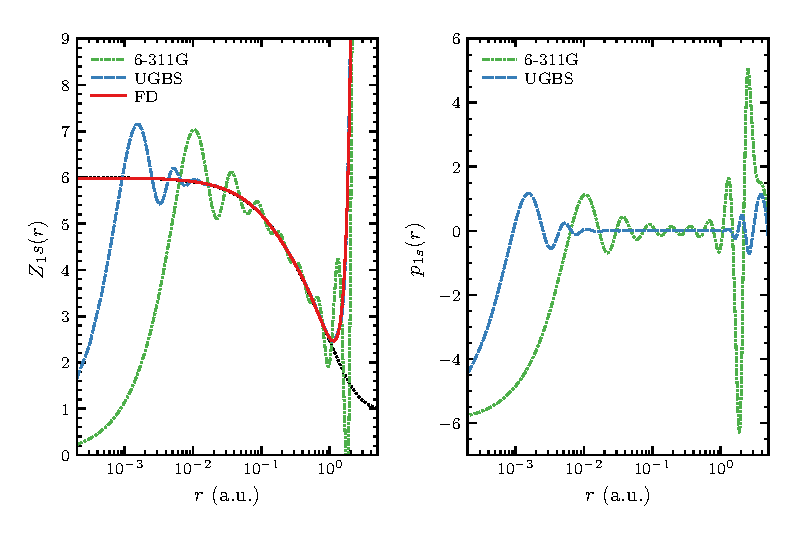
\includegraphics[width=0.9\textwidth]{dim/carbon_prof.eps}
\caption[Inversión de orbitales descritos con conjuntos de base finitos.]
{(a) Cargas efectivas invertidas del orbital $1s$ del átomo de carbón.
(b)~Perfiles de oscilación de los conjuntos de base.}
\label{fig:1sCarbon}
\end{figure}

Para ilustrar este procedimiento, se considera el orbital $1s$ del átomo 
de carbono. Primero, se resuelven las ecuaciones de Hartree--Fock usando 
el conjunto de bases \mbox{6-311G} con el código 
\textsc{gamess}~\cite{Schmidt:93,Gordon:05}. Luego, aplicando la 
Ec.~(\ref{eq:Vinv}), se obtiene la carga invertida correspondiente. La 
carga resultante $Z_{1s}^{\mbox{\scriptsize 6-311G}}$ se muestra en la 
Fig.~\ref{fig:1sCarbon}(a) con una línea raya-punto. La carga tiene  
oscilaciones en toda su extensión radial, divergiendo para valores 
grandes de $r$. Se realiza el mismo cálculo con el conjunto de base 
universal Gaussiano (\acs{ugbs}), que tiene un número significativamente 
mayor de funciones primitivas. La carga invertida correspondiente 
$Z_{1s}^{\mbox{\scriptsize UGBS}}$ se presenta en la figura con una 
línea discontinua. A pesar que la carga aún diverge cerca de 
$r\approx1\,$a.u., las oscilaciones ahora están circunscriptas cerca del 
núcleo. Finalmente, se resuelven las ecuaciones diferenciales de 
Hartree--Fock para el átomo de carbono usando el método de diferencias 
finitas (\acs{fd}) con el código \textsc{hf} de C. Froese 
Fischer~\cite{FroeseFischer:97}. La carga invertida 
$Z_{1s}^{\mbox{\scriptsize FD}}$ correspondiente se 
exhibe con una línea sólida en la Fig.~\ref{fig:1sCarbon}(a). Como es de 
esperar, esta carga invertida no presenta oscilaciones, ya que no se 
utilizó una base para construir los orbitales. Sin embargo, la carga 
diverge para $r>1\,$a.u. debido a las características de la teoría de 
Hartree--Fock que se detallan en la Sección~\ref{sec:discusionHF}. En el 
caso del carbono, los conjuntos de base considerados para calcular el 
orbital $1s$ fueron \mbox{6-311G} y UGBS. Los perfiles de oscilación 
correspondientes, usando la Ec.~(\ref{eq:oscillation-prof}), se muestran 
en la Fig.~\ref{fig:1sCarbon}(b). Dado que los perfiles de oscilación 
para cada conjunto de base son característicos, una vez determinados, 
éstos se sustraen de los potenciales moleculares invertidos de manera 
directa. Luego, se implementa la Ec.~(\ref{eq:molzDIM}) y los parámetros 
se optimizan siguiendo la metodología presentada en la 
Sección~\ref{sec:dimatomos}.

%%%%%%%%%%%%%%%%%%%%%%%%%%%%%%%%%%%%%%%%%%%%%%%%%%%%%%%%%%%%%%%%%%%%%%%%
\section{Resultados}
%%%%%%%%%%%%%%%%%%%%%%%%%%%%%%%%%%%%%%%%%%%%%%%%%%%%%%%%%%%%%%%%%%%%%%%%
\label{sec:dimresultados}

En esta Sección se presentan los resultados obtenidos mediante la  
implementación del método de inversión depurada para describir blancos
atómicos y moleculares. El DIM se combina con la primera aproximación de 
Born para describir la ionización por impacto de protones y fotones en 
estos blancos multielectrónicos. Las secciones eficaces de ionización 
predichas por el modelo DIM-FBA se examinan mediante comparación con los 
datos experimentales disponibles. En total, se presentan 
resultados de cuatro blancos: helio, nitrógeno, neón y metano. Sin 
embargo, una gran cantidad de potenciales DIM se han presentado en 
diversas publicaciones en los últimos años~\cite{Mendez:16,Mendez:19dim,
Mendez:18}. Además, actualmente se está trabajando en una base de datos 
de estructura de átomos y potenciales que cubre todos los elementos no 
relativistas de la tabla periodica, que será de libre acceso.

%%%%%%%%%%%%%%%%%%%%%%%%%%%%%%%%%%%%%%%%%%%%%%%%%%%%%%%%%%%%%%%%%%%%%%%%
\subsection{Estructura electrónica de blancos}
%%%%%%%%%%%%%%%%%%%%%%%%%%%%%%%%%%%%%%%%%%%%%%%%%%%%%%%%%%%%%%%%%%%%%%%%
\label{subsec:dimtarget}

Las soluciones $u_{nl}^{\mathrm{HF}}$ y $\varepsilon^{\mathrm{HF}}$ de 
Hartree--Fock que se implementan en la Ec.~(\ref{eq:Vinv}) se calculan 
usando los códigos \textsc{hf} de C. Froese 
Fischer~\cite{FroeseFischer:97}, 
y \textsc{nrhf} de W. Johnson~\cite{Johnson:07}. Un aspecto importante 
del DIM está dado por la autoconsistencia de los códigos numéricos 
usados. Se estudiaron los códigos fuentes de ambas implementaciones y se 
emplearon los mismas grillas y métodos numéricos, tanto en la inversión 
como en la optimización de los potenciales.

%=======================================================================
\subsubsection*{Helio}
%=======================================================================

En primer lugar, se muestran los resultados obtenidos de implementar
el método de inversión depurada en el átomo de helio en su estado
fundamental. La inversión del orbital $1s$ no presenta ningún defecto
de los descritos en la Sección~\ref{subsec:invHF}. Además, la 
simplicidad del átomo de helio nos permite ajustar la carga invertida 
con un número reducido de parámetros. La carga invertida 
$Z_{1s}^{\mathrm{HF}}$ y la carga invertida depurada 
$Z_{1s}^{\mathrm{DIM}}$ se muestran en la Fig.~\ref{fig:Hepots}(a) con 
línea discontinua y sólida, respectivamente. La carga DIM descrita por 
la Ec.~(\ref{eq:atomzDIM}), se optimiza con sólo tres parámetros, los 
cuales se dan en la Tabla~\ref{tab:params-atoms}. 

\begin{figure}[t]
\centering
\includegraphics[width=0.9\textwidth]{figures/dim/Hepots.eps}
\caption[Cargas efectivas y potencial de intercambio DIM de He.]
{(a) Cargas efectivas $1s$ del He ($^1$S) obtenidas mediante inversión 
directa (línea discontinua) e inversión depurada (línea sólida). 
(b) Potencial de intercambio DIM (línea sólida) y OPM (línea punteada).}
\label{fig:Hepots}
\end{figure}

Para verificar la calidad de la estructura atómica dada por el potencial 
DIM, en la Tabla~\ref{tab:results-atoms} se presenta una comparación 
de los valores de energías total, orbital y radios medios obtenidos 
utilizando el método de inversión depurada (fila superior) con sus 
correspondientes valores de Hartree--Fock (fila inferior). El potencial 
DIM reproduce el valor de energía total, dada por la 
Ec.~\ref{eq:Etotal}, en un $0.003\%$. La energía orbital $1s$ coincide 
con la energía de HF en 6 cifras significativas. Los valores medios de 
$u_{1s}^{\mathrm{DIM}}$ también muestran una excelente concordancia, 
tanto para la región cercana al origen, $\langle 1/r\rangle$, como en la 
región lejana, $\langle r\rangle$.

El potencial de intercambio orbital DIM del átomo de helio, definido por 
la Ec.~\ref{eq:exchange-potential}, se muestra en la 
Fig.~\ref{fig:Hepots}(b). También se muestran los valores del 
\textit{optimized potential method} (\acs{opm}), que se obtienen a 
partir del código \textsc{atomopm} de Talman~\cite{Talman:76,Talman:89}. 
Los potenciales DIM y OPM coinciden en todo el rango de $r$. Las 
energías total y orbital de intercambio, dadas por la 
Ec.~(\ref{eq:exchange-energy}), del estado fundamental del helio se 
presentan en la Tabla~\ref{tab:exchange-atoms}. La energía total 
concuerda muy bien con el valor de intercambio exacto atómico de 
Hartree--Fock (EAHF, por sus siglas en inglés)~\cite{Becke:88}.

%=======================================================================
\subsubsection*{Nitrógeno}
%=======================================================================

Los excelentes resultados obtenidos a partir de la implementación de DIM 
en el átomo de helio pueden atribuirse a la simplicidad del orbital y su 
simetría esférica. Para evaluar la capacidad del DIM para describir 
blancos con más electrones y de capa abierta, a continuación, se 
considera el átomo de nitrógeno. 

\begin{figure}[t]
\centering
\includegraphics[width=0.9\textwidth]{figures/dim/N4S_DIM.eps}
\caption[Cargas efectivas DIM de N.]
{Cargas efectivas $1s$, $2s$ y $2p$ del término $^4$S de N obtenidas 
mediante inversión directa (líneas discontinuas) e inversión depurada 
(líneas sólidas).}
\label{fig:Nzeff}
\end{figure}

\begin{figure}[t]
\centering
\includegraphics[width=0.9\textwidth]{figures/dim/N_Vx.eps}
\caption[Potenciales de intercambio DIM de N.]
{Potenciales de intercambio DIM de los términos $^4$S (línea sólida), 
$^2$D (línea discontinua) y $^2$P (línea punto-raya), y valores OPM 
(línea punteada) de N.}
\label{fig:NVx}
\end{figure}

La configuración electrónica del estado fundamental del nitrógeno $2p^3$ 
da lugar a tres términos: $^4$S, $^2$D y $^2$P. Cada uno de estos 
términos está descrito por una densidad electrónica diferente. En la 
Fig.~\ref{fig:Nzeff} se muestran las cargas de los orbitales $1s$, $2s$ 
y $2p$ obtenidas a partir de la inversión directa (líneas discontinuas) 
y el método de inversión depurada (líneas continuas) del término de 
energía más bajo de N. La inversión del orbital $u_{1s}^{\mathrm{HF}}$ 
diverge en la región asintótica, mientras que el nodo genuino del 
orbital $2s$, en $r\approx 0.32$~a.u., resulta en un polo. 

La implementación del método de inversión depurada permite ajustar 
analíticamente la carga invertida en el mayor rango posible. Luego de 
una optimización cuidadosa del blanco, se obtienen los parámetros de las 
cargas DIM correspondientes a los términos $^4$S, $^2$D y $^2$P, que se 
dan en la Tabla~\ref{tab:params-atoms}. Las soluciones obtenidas de 
resolver la Ec.~(\ref{eq:eqSchroRadial}) con los potenciales DIM de N 
se presentan en la Tabla~\ref{tab:results-atoms}. Las energías totales, 
orbitales y valores radiales medios se reproducen hasta en un $0.05\%$, 
$1\times 10^{-4}\%$ y $0.3\%$ los valores HF, respectivamente. 

En la Fig.~\ref{fig:NVx} se muestran los potenciales de intercambio 
$1s$, $2s$ y $2p$ de los términos $^4$S (línea sólida), $^2$D (línea 
discontinua) y $^2$P (línea raya-punto) de N. Los potenciales 
$V_{nl}^{\mathrm{x}}$ se comparan con el potencial de intercambio OPM 
(línea punteada). Los potenciales de intercambio del orbital $1s$ de 
cada término se comportan de manera similar. El potencial OPM sigue a 
los valores DIM cerca del origen y asintóticamente. En el caso del 
orbital $2s$, los potenciales de intercambio correspondientes a cada 
término se comportan de manera diferente en el origen. Para valores 
$r>0.5$~a.u., los potenciales DIM y OPM convergen. Nótese que el 
potencial OPM concuerda muy bien con el potencial $V_{2s}^{\mathrm{x}}$ 
del término $^2$D. Finalmente, los potenciales de intercambio DIM $2p$ 
también se comportan de manera similar entre sí. Sin embargo, los 
potenciales DIM y OPM convergen sólo en la región asintótica. Es notable 
como el potencial, que no es orbital, tiende a seguir el comportamiento 
de los potenciales orbitales DIM a lo largo de $r$. 

Los valores de energía de intercambio orbitales y total de los tres 
términos del estado fundamental de N se muestran en la 
Tabla~\ref{tab:exchange-atoms}. La energía de intercambio orbital $1s$ 
de todos los términos son iguales, como se esperaría para un orbital de 
capa cerrada. De manera similar, las energías correspondientes al 
orbital $2s$ varían ligeramente, con una dispersión del $0.08\%$. Esta 
desviación se debe al comportamiento distintivo de cada potencial cerca 
del origen. Dado que la capa $2p$ está abierta, la energía de 
intercambio del orbital $2p$ varía significativamente en los diferentes 
términos, con una dispersión de hasta 18\%. 
A partir de la Ec.~(\ref{eq:exchange-energy}), se calculan las energías 
de intercambio total. La energía del término más bajo y el valor EAHF 
presenta un acuerdo cercano al $0.1\%$.

%=======================================================================
\subsubsection*{Neón}
%=======================================================================

La implementación del DIM en neón es análoga al caso de nitrógeno. Esta
vez, la capa de valencia del átomo está llena. Los resultados de la 
optimización de los parámetros que definen las cargas efectivas, dadas 
por la Ec.~(\ref{eq:atomzDIM}), del átomo de neón se muestran en la 
Tabla~\ref{tab:params-atoms}. La comparación entre las soluciones de los 
potenciales DIM y el método de Hartree--Fock se dan en la 
Tabla~\ref{tab:results-atoms}. El acuerdo en energías orbitales es 
excelente, del orden de $1\times 10^{-5}$, mientras que DIM reproduce 
los valores medios de los orbitales HF en aproximadamente $0.1\%$. Por 
otro lado, la energía total tiene una dispersión del $0.04\%$ respecto 
a HF. Las energías de intercambio total y orbitales que se obtienen a 
partir del DIM se presentan en la Tabla~\ref{tab:exchange-atoms}. Las 
energías $E^{\mathrm{x}}$ y los valores EAHF acuerdan en $0.04\%$.

%%%%%%%%%%%%%% RESULTADOS %%%%%%%%%%%%%%
\begin{table}
\begin{center}
\begin{tabular}{
>{\centering\arraybackslash}p{0.12\textwidth}
>{\centering\arraybackslash}p{0.05\textwidth}
>{\centering\arraybackslash}p{0.22\textwidth}
>{\centering\arraybackslash}p{0.22\textwidth}
>{\centering\arraybackslash}p{0.22\textwidth}}
\rowcolor{mydarkgray} 
   &       & $nl$ & $z_j$        & $\alpha_j$   \\
%%%%%%%%%%%%%%%%%%%% Helio %%%%%%%%%%%%%%%%%%%%
He & $^1$S & $1s$ &  $1.3175$ & $2.5003$  \\\rowcolor{mygray} 
   &       &      & $-0.3175$ & $5.0437$  \\ 
%%%%%%%%%%%%%%%%%% Nitrogeno %%%%%%%%%%%%%%%%%%
N  & $^4$S & $1s$ & $5.2563$ & $1.2621$  \\\rowcolor{mygray} 
   &       &      & $0.7437$ & $8.0284$  \\ 
   &       & $2s$ & $2.7136$ & $0.8947$ \\\rowcolor{mygray} 
   &       &      & $2.4528$ & $3.5127$  \\
   &       &      & $0.8336$ & $3.3865$  \\ \rowcolor{mygray} 
   &       & $2p$ & $3.6435$ & $1.2407$  \\ 
   &       &      & $2.0550$ & $5.3514$  \\\rowcolor{mygray} 
   &       &      & $0.3015$ & $0.2866$ \\
   & $^2$D & $1s$ & $5.1664$ & $1.2241$  \\\rowcolor{mygray} 
   &       &      & $0.8137$ & $7.5680$  \\ 
   &       & $2s$ & $3.7478$ & $2.8531$  \\\rowcolor{mygray} 
   &       &      & $1.8541$ & $1.0311$  \\ 
   &       &      & $0.3981$ & $0.2397$ \\\rowcolor{mygray} 
   &       & $2p$ & $4.0105$ & $1.2874$  \\ 
   &       &      & $1.8552$ & $5.7086$  \\\rowcolor{mygray} 
   &       &      & $0.1343$ & $0.2680$ \\
   & $^2$P & $1s$ & $5.1864$ & $1.2178$  \\\rowcolor{mygray} 
   &       &      & $0.8137$ & $7.5674$  \\ 
   &       & $2s$ & $3.6700$ & $3.1495$  \\\rowcolor{mygray} 
   &       &      & $1.4394$ & $0.7404$  \\ 
   &       &      & $0.8907$ & $0.8306$ \\\rowcolor{mygray} 
   &       & $2p$ & $2.3280$ & $1.4093$  \\ 
   &       &      & $1.8977$ & $1.1656$  \\\rowcolor{mygray} 
   &       &      & $1.7743$ & $5.6878$ \\
%%%%%%%%%%%%%%%%%%%%%%%%%%%%%%%%%%%%%%%%%%%%%%%
Ne & $^1$S & $1s$ & $7.3677$ & $2.4173$ \\\rowcolor{mygray} 
   &       &      & $1.3004$ & $0.1264$ \\
   &       &      & $0.3320$ & $13.1582$ \\\rowcolor{mygray} 
   &       & $2s$ & $0.2977$ & $17.9939$ \\
   &       &      & $0.6681$ & $0.0673$ \\\rowcolor{mygray} 
   &       &      & $8.0342$ & $2.4722$ \\
   &       & $2p$ & $1.3531$ & $8.5695$ \\\rowcolor{mygray} 
   &       &      & $0.3359$ & $0.4649$ \\
   &       &      & $7.3111$ & $2.0906$ \\
\end{tabular}
\caption[Parámetros de la carga efectiva de He, N y Ne.]
{Parámetros de la carga efectiva $Z_{1s}^{\mathrm{ DIM}}$ de He ($^1$S), 
N ($^4$S, $^2$D, $^2$P) y Ne ($^1$S).}
\label{tab:params-atoms}
\end{center}
\end{table}

\begin{table}
\begin{center}
\begin{tabular}{
>{\centering\arraybackslash}p{0.07\textwidth}
>{\centering\arraybackslash}p{0.03\textwidth}
>{\centering\arraybackslash}p{0.15\textwidth}
>{\centering\arraybackslash}p{0.10\textwidth}
>{\centering\arraybackslash}p{0.15\textwidth}
>{\centering\arraybackslash}p{0.15\textwidth}
>{\centering\arraybackslash}p{0.15\textwidth}}
\rowcolor{mydarkgray} 
   & & $E$ & $nl$ & $\varepsilon_{nl}$ & $\left<r\right>_{nl}$ & $\left<1/r\right>_{nl}$ \\
He & $^1$S & $-2.8616$   & $1s$ & $-0.9180$  & $0.9273$ & $1.6873$ \\\rowcolor{mygray} 
   &       & $-2.8617$   &      & $-0.9180$  & $0.9273$ & $1.6873$ \\
N  & $^4$S & $-54.3762$  & $1s$ & $-15.6291$ & $0.2283$ & $6.6487$ \\\rowcolor{mygray} 
   &       & $-54.4009$  &      & $-15.6291$ & $0.2283$ & $6.6532$ \\
   &       &             & $2s$ & $-0.9453$  & $1.3345$ & $1.0804$ \\\rowcolor{mygray} 
   &       &             &      & $-0.9453$  & $1.3323$ & $1.0782$ \\
   &       &             & $2p$ & $-0.5676$  & $1.4127$ & $0.9550$ \\\rowcolor{mygray} 
   &       &             &      & $-0.5676$  & $1.4096$ & $0.9577$ \\
   & $^2$D & $-54.2756$  & $1s$ & $-15.6664$ & $0.2283$ & $6.6493$ \\\rowcolor{mygray} 
   &       & $-54.2962$  &      & $-15.6664$ & $0.2283$ & $6.6539$ \\
   &       &             & $2s$ & $-0.9637$  & $1.3292$ & $1.0874$ \\\rowcolor{mygray} 
   &       &             &      & $-0.9637$  & $1.3263$ & $1.0832$ \\
   &       &             & $2p$ & $-0.5087$  & $1.4488$ & $0.9388$ \\\rowcolor{mygray} 
   &       &             &      & $-0.5087$  & $1.4466$ & $0.9421$ \\
   & $^2$P & $-54.2086$  & $1s$ & $-15.6916$ & $0.2282$ & $6.6504$ \\\rowcolor{mygray} 
   &       & $-54.2281$  &      & $-15.6916$ & $0.2282$ & $6.6543$ \\
   &       &             & $2s$ & $-0.9763$  & $1.3256$ & $1.0871$ \\\rowcolor{mygray} 
   &       &             &      & $-0.9763$  & $1.3223$ & $1.0866$ \\
   &       &             & $2p$ & $-0.4713$  & $1.4718$ & $0.9298$ \\\rowcolor{mygray} 
   &       &             &      & $-0.4713$  & $1.4730$ & $0.9316$ \\
Ne & $^1$S & $-128.4978$ & $1s$ & $-32.7725$ & $0.1575$ & $9.6215$ \\\rowcolor{mygray} 
   &       & $-128.5475$ &      & $-32.7724$ & $0.1576$ & $9.6181$ \\
   &       &             & $2s$ & $-1.9304$  & $0.8913$ & $1.6408$ \\\rowcolor{mygray} 
   &       &             &      & $-1.9304$  & $0.8921$ & $1.6326$ \\  
   &       &             & $2p$ & $-0.8504$  & $0.9678$ & $1.4303$ \\\rowcolor{mygray} 
   &       &             &      & $-0.8504$  & $0.9653$ & $1.4354$ \\
\end{tabular}
\caption[Energías y radios medios de He, N y Ne.]
{Energías totales, energías orbitales y radios medios de He ($^1$S), 
N ($^4$S, $^2$D, $^2$P) y Ne ($^1$S) obtenidos con el método de 
inversión depurada (filas superiores) y con el método de HF (filas 
inferiores).}
\label{tab:results-atoms}
\end{center}
\end{table}

\begin{table}
\begin{center}
\begin{tabular}{
>{\centering\arraybackslash}p{0.07\textwidth}
>{\centering\arraybackslash}p{0.03\textwidth}
>{\centering\arraybackslash}p{0.14\textwidth}
>{\centering\arraybackslash}p{0.14\textwidth}
>{\centering\arraybackslash}p{0.14\textwidth}
>{\centering\arraybackslash}p{0.14\textwidth}
>{\centering\arraybackslash}p{0.14\textwidth}}
\rowcolor{mydarkgray} 
   &      & $1s$     & $2s$     & $3s$     & Total    & EAHF~\cite{Becke:88} \\
He & $^1$S & $-0.5129$ &           &           & $-1.0258$ & $-1.026$ \\\rowcolor{mygray} 
N  & $^4$S & $-2.1175$ & $-0.4776$ & $-0.4711$ & $-6.6034$ & $-6.596$ \\
   & $^2$D & $-2.1175$ & $-0.4777$ & $-0.4262$ & $-6.4688$ & \\\rowcolor{mygray} 
   & $^2$P & $-2.1175$ & $-0.4780$ & $-0.3973$ & $-6.3827$ & \\
Ne & $^1$S & $-3.1106$ & $-0.8620$ & $-0.6938$ & $-12.1080$ & $-12.105$ \\\rowcolor{mygray} 
\end{tabular}
\caption[Energías de intercambio total y orbitales de He, N y Ne.]
{Energías de intercambio total y orbitales DIM de He ($^1$S), N ($^4$S, 
$^2$D, $^2$P) y Ne ($^1$S).}
\label{tab:exchange-atoms}
\end{center}
\end{table}

%=======================================================================
\subsubsection*{Metano}
%=======================================================================

El método de inversión depurada para sistemas moleculares se aplica a 
la molécula de metano. Este hidruro es altamente simétrico y, por lo 
tanto, puede ser descrito por un potencial angular 
promediado~\cite{Granados:16}. 

\begin{figure}[t]
\centering
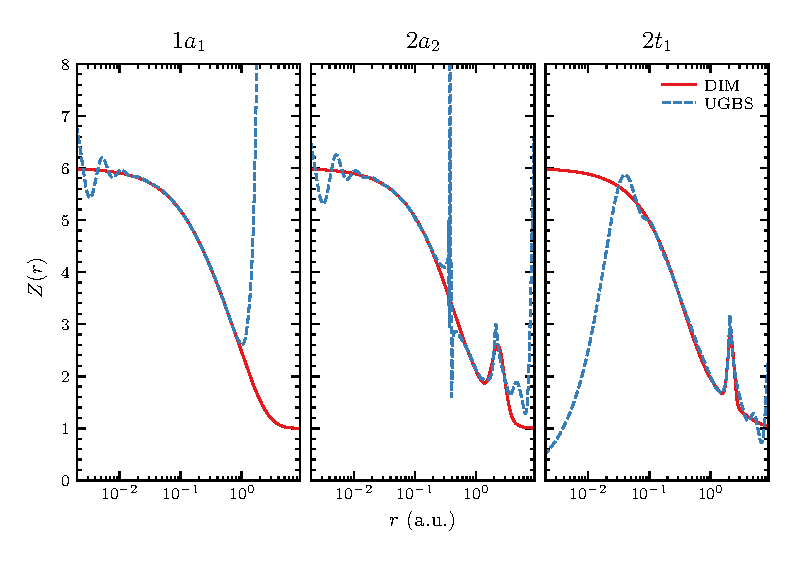
\includegraphics[width=0.9\textwidth]{figures/dim/ch4_dim.eps}
\caption[Cargas invertidas y depuradas de metano.]
{Cargas efectivas de CH$_4$ de los orbitales moleculares $1a_1$, $2a_2$ 
y $2t_1$ obtenidas a partir del conjunto de base UGBS; inversión directa 
(líneas discontinuas) e inversión depurada (líneas sólidas).}
\label{fig:ch4zeff}
\end{figure}

Los orbitales moleculares HF de CH$_4$ se calculan usando los conjuntos 
de bases UGBS del carbono y el hidrógeno. Estas bases sólo consideran 
momentos angulares hasta $L=1$. El cálculo de estructura electrónica de 
metano con estos conjuntos de base deberían incluir funciones de 
polarización (por lo menos hasta las funciones $d$), con el fin de 
incrementar la precisión de las energías moleculares~\cite{Rothenberg:71,
Hariharan:72}. Sin embargo, para aislar los efectos de la base, éstos 
efectos no se incluyen aquí. 

Las cargas obtenidas mediante la inversión directa de los orbitales UGBS 
se muestran en la Fig.~\ref{fig:ch4zeff} con líneas discontinuas. Dado 
que los orbitales moleculares se describen a partir de combinaciones 
lineales de orbitales atómicos de hidrógeno y carbono, para remover los 
efectos de las bases, se deben determinar los perfiles de oscilación de 
de cada uno de los átomos constituyentes. Se emplea la 
Ec.~(\ref{eq:oscillation-prof}) para determinar los perfiles 
$p_{1s}^{\mbox{\scriptsize UGBS}}$, $p_{2s}^{\mbox{\scriptsize UGBS}}$ y 
$p_{2p}^{\mbox{\scriptsize UGBS}}$ del carbono. Así, se sustraen los 
perfiles $p_{nl}^{\mbox{\scriptsize UGBS}}$ de las correspondientes 
cargas invertidas $Z_{nl}^{\mbox{\scriptsize UGBS}}$ del metano. Las 
oscilaciones se remueven completamente para todos los orbitales excepto 
el $2a_2$, que presenta pequeñas fluctuaciones residuales debido a la 
base del hidrógeno. Ya que estas ondulaciones son mínimas y se ubican 
cerca del núcleo, éstas pueden ser despreciadas y se procede a 
implementar el método de depuración descrito en la 
Sección~\ref{sec:dimmoleculas}. 

Los parámetros de las cargas moleculares DIM definidos por la 
Ec.~(\ref{eq:molzDIM}) se presentan en la Tabla~\ref{tab:ch4parameters}. 
Las cargas correspondientes se muestran en la Fig.~\ref{fig:ch4zeff} con 
líneas sólidas. En este caso, la función de costo~(\ref{eq:fncosto-dim}) 
que se minimiza considera los valores de energía y radios medios de los 
MOs dados por Moccia~\cite{Moccia:69}. Las energías orbitales reproducen 
las originales hasta la cuarta cifra significativa y se dan en la 
Tabla~\ref{tab:ch4parameters}. Por otro lado, los radios medios 
$\langle r\rangle$ y $\langle 1/r\rangle$ obtenidos con los potenciales 
moleculares DIM están dentro del $1\%$ de los valores de Moccia.

\begin{table}[t]
\centering
\begin{tabular}{
>{\centering\arraybackslash}p{0.13\textwidth}
>{\centering\arraybackslash}p{0.13\textwidth}
>{\centering\arraybackslash}p{0.13\textwidth}
>{\centering\arraybackslash}p{0.13\textwidth}
>{\centering\arraybackslash}p{0.13\textwidth}
>{\centering\arraybackslash}p{0.13\textwidth}}
\rowcolor{mydarkgray} 
   $nl$ & $E$        & $z_j$        & $\alpha_j$   & $\beta$ & $\gamma$ \\
$1a_1$  & $-11.1949$ & $1.925280$ & $0.641982$ & & \\
\rowcolor{mygray} 
        &            & $0.953120$ & $5.571510$ & & \\
        &            & $2.121600$ & $1.500440$ & & \\
\rowcolor{mygray} 
$2a_2$  & $-0.9204$  & $2.912200$ & $3.149990$ & & \\
        &            & $2.087800$ & $0.771371$ & & \\
\rowcolor{mygray} 
        &            & $1.23640$  &            & $2.329570$ & $0.053420$ \\
$2t_1$  & $-0.5042$  & $0.901953$ & $2.895140$ & & \\
\rowcolor{mygray} 
        &            & $1.112030$ & $0.388649$ & & \\
        &            & $2.986017$ & $2.931210$ & & \\
\rowcolor{mygray} 
        &            & $1.301820$ &            & $2.169850$ & $0.012616$ \\ 
\end{tabular}
\caption[Energías y parámetros de ajuste de cargas efectivas de metano.]
{Energías orbitales moleculares y parámetros de ajuste de cargas 
efectivas de metano.}
\label{tab:ch4parameters}
\end{table}

%%%%%%%%%%%%%%%%%%%%%%%%%%%%%%%%%%%%%%%%%%%%%%%%%%%%%%%%%%%%%%%%%%%%%%%%
\subsection{Procesos colisionales simples}
%%%%%%%%%%%%%%%%%%%%%%%%%%%%%%%%%%%%%%%%%%%%%%%%%%%%%%%%%%%%%%%%%%%%%%%%
\label{subsec:procol}

En esta Sección se analiza la respuesta de los potenciales efectivos 
DIM obtenidos en la Sección~\ref{subsec:dimtarget} mediante el método 
de inversión depurada para helio, nitrógeno, neón y metano.
En los blancos moleculares, la orientación molecular es importante para 
determinar la sección eficaz en un proceso colisional. Sin embargo, en 
la configuración experimental, las moléculas en estado gaseoso 
generalmente tienen orientaciones aleatorias. Por lo tanto, la 
descripción promediada esféricamente de los sistemas moleculares asumida 
por el potencial DIM está en concordancia con la configuración del 
blanco. Los procesos colisionales que se examinan en esta Sección se 
describen a primer orden empleando la primera aproximación de Born 
(FBA). La combinación de la descripción del blanco mediante el potencial 
efectivo DIM y el modelado de la fotoionización a primer orden se 
denomina como ionización DIM-FBA. 

%=======================================================================
\subsubsection{Fotoionización}
%=======================================================================

Las secciones eficaces de ionización simple por impacto de fotón 
resultantes de la implementación del DIM en combinación con la FBA para 
helio, nitrógeno, neón y metano se muestran en la 
Fig.~\ref{fig:photoDIM} con líneas sólidas. Los resultados teóricos 
DIM-FBA para helio y nitrógeno coinciden de manera excelente con los 
valores experimentales (símbolos)~\cite{Samson:90,Henke:93,Stolte:16} a 
bajas, medias y altas energías del fotón incidente. En el caso del átomo 
de neón, algunas discrepancias con las mediciones (símbolos) 
\cite{Henke:93,Samson:02} empiezan a surgir a energías bajas e 
intermedias del proyectil. Este comportamiento sugiere la necesidad de 
incluir en la descripción de la fotoionización correcciones de mayor 
orden que incluyan efectos de múltiples cuerpos que puedan ser 
relevantes, tales como la relajación de los orbitales debido a la 
creación de un hueco electrónico, respuestas colectivas de electrones 
de capas internas~\cite{Ederer:64} y efectos de correlación.

\begin{figure}
\centering
\includegraphics[width=0.92\textwidth]{dim/fotoDIM-part1.eps} 

\vspace{-1.15cm}
\includegraphics[width=0.92\textwidth]{dim/fotoDIM-part2.eps}
\caption[Fotoionización de He, N, Ne y CH$_4$.]
{Sección eficaz total de fotoionización de un electrón de He, N, Ne y 
CH$_4$. Curvas: cálculos teóricos DIM-FBA. Símbolos: 
datos experimentales~\cite{Samson:90,Henke:93,Stolte:16,Samson:02,
Lukirskii:64,Henke:82,Samson:89}.}
\label{fig:photoDIM}
\end{figure}

La predicción del modelo DIM-FBA para la sección eficaz total de 
fotonización de CH$_4$ se encuentra en buen acuerdo con valores 
experimentales en el rango de altas energías y cerca del umbral. La 
curva entre aproximadamente 15 y 300 eV muestra la fotoionización de la 
capa de valencia, mientras que la discontinuidad en $0.3$~keV 
corresponde al umbral del orbital molecular $1a_1$. Para fotoenergías 
bajas e intermedias, el acuerdo entre las predicciones DIM-FBA y los 
datos experimentales~\cite{Lukirskii:64,Henke:82,Samson:89} no es bueno. 
Fenónemos tales como la relajación de los orbitales moleculares, 
posibles contribuciones colectivas y efectos de correlación deben ser  
considerados en futuros cálculos. Por otro lado, para la fotoionización 
de un electrón perteneciente al orbital interno $1a_1$, estos efectos no 
son tan signficativos, y se tiene buen acuerdo con los valores 
experimentales disponibles. 

%=======================================================================
\subsubsection{Ionización por impacto de protones}
%=======================================================================

\begin{figure}
\centering
\includegraphics[width=0.9\textwidth]{figures/dim/ionDIM.eps}
\caption[Ionización por impacto de protón de N y CH$_4$.]
{Sección eficaz total de ionización de un electrón por impacto de protón 
de N y CH$_4$. Línea sólida: cálculos teóricos DIM-FBA. 
Símbolos: datos experimentales de ionización por impacto de 
protón~\cite{Rudd:83,Rudd:85} y electrón~\cite{Brook:78} con conversión 
de equivelocidad.}
\label{fig:iondim}
\end{figure}

Los resultados de ionización por impacto de protón en N y CH$_4$, 
en el marco del modelo DIM-FBA, se muestra en la Fig.~\ref{fig:iondim}. 
El acuerdo entre las predicciones teóricas y las datos 
experimentales~\cite{Rudd:83,Rudd:85} es muy bueno en la región de altas 
energías, donde tiene validez la primera aproximación de Born. En el 
caso de nitrógeno, incluimos también datos experimentales de ionización 
por impacto de electrón~\cite{Brook:78}. Para valores de energía mayores 
a 400~keV, la sección eficaz de ambos proyectiles coincide. 

%%%%%%%%%%%%%%%%%%%%%%%%%%%%%%%%%%%%%%%%%%%%%%%%%%%%%%%%%%%%%%%%%%%%%%%%
\section{Conclusiones}
%%%%%%%%%%%%%%%%%%%%%%%%%%%%%%%%%%%%%%%%%%%%%%%%%%%%%%%%%%%%%%%%%%%%%%%%
\label{sec:conclu-dim}

En este Capítulo se desarrolló el método de inversión depurada (DIM) 
para obtener potenciales efectivos que permitan describir la estructura 
electrónica de blancos atómicos y moleculares de manera precisa. La 
disponibilidad de estos potenciales permite conocer los estados 
iniciales y finales del blanco en una colisión de manera directa. 

El método de inversión depurada es general y aplicable a soluciones que 
se obtienen en el marco de diversas aproximaciones. En este trabajo se 
mostró la implementación del DIM a partir de soluciones dadas por la 
teoría de Hartree--Fock. Los potenciales resultantes de la inversión de 
orbitales HF presentan defectos numéricos (polos y divergencias).
%Los potenciales DIM se obtienen a partir de la inversión de ecuaciones 
%de un electrón con soluciones de Hartree--Fock. Los potenciales 
%resultantes presentan defectos numéricos (polos y divergencias), los 
%cuales son examinados en detalle. Se encuentra que los defectos están 
%dados por características de la teoría de Hartree--Fock no compatibles
%con la inversión. Los polos se deben a nodos genuinos de los orbitales 
%HF que no son puntos de inflexión. Si bien esta característica de los 
%orbitales no es explícita en la teoría, la obtención de potenciales sin 
%polos así lo requiere. Las divergencias asintóticas del potencial se 
%deben al coeficiente del decaimiento exponencial de los orbitales HF. 
%La teoría de HF establece que éstos decaen con la energía del HOMO. Sin 
%embargo, la obtención de potenciales con correcto comportamiento 
%asintótico mediante el esquema de inversión requiere que cada orbital 
%decaiga con la energía del dicho orbital. También se encontraron 
%oscilaciones en los orbitales de las capas internas de átomos con carga 
%nuclear $Z\ge 12$, que dan lugar a nodos espurios. Estas oscilaciones 
%parecen surgir debido al término de intercambio a grandes distancias. 
Siguiendo el método de depuración, los defectos encontrados en la 
inversión se descartan y las cargas invertidas se ajustan con una 
expresión analítica simple. Los parámetros que definen esta expresión 
son optimizados cuidadosamente hasta reproducir las soluciones iniciales.
A modo de corolario, y dado que la teoría de Hartree--Fock contiene el 
término de intercambio de forma exacta, se definieron potenciales de 
intercambio orbitales ``exactos''. También se dieron ecuaciones para la 
energía total del sistema, energías de intercambio orbitales y totales.
Luego, el método de inversión depurada diseñada para átomos se extendió 
para moléculas. Debido a que los orbitales moleculares se expresan a 
partir de conjuntos de base finitas, las soluciones presentan 
ondulaciones casi imperceptiles. La implementación de la inversión 
traduce estas pequeñas fluctuaciones como grandes oscilaciones en la 
carga molecular. Debido a esto, se requieren pasos adicionales en el 
método de depuración, los cuales incluyen la determinación de perfiles 
de oscilación de los conjuntos de base atómicas utilizadas en el cálculo 
molecular. 

Se implementó el método DIM para obtener potenciales efectivos y de 
intercambio que reproducen las soluciones de HF de forma precisa en tres 
blancos atómicos: helio, nitrógeno y neón. Además, se empleó el método 
DIM extendido a moléculas para describir la molécula de metano. Las 
soluciones que se obtienen de estos potenciales reproducen los valores
originales con gran precisión. 

La efectividad del DIM para describir la estructura de blancos en una 
colisión fue examinado a partir de la primera aproximación de Born. Los 
potenciales de He, N, Ne y CH$_4$ se implementaron para calcular, en 
conjunción con la FBA, secciones eficaces de ionización por el impacto 
de protones y fotones. En términos generales, ambos procesos se 
reproducen con buena concordancia los datos experimentales disponibles. 
Las discrepancias principales se atribuyen al hecho de que el modelo 
teórico sólo considera el primer orden perturbativo. Será necesario 
implementar métodos perturbativos con mayor orden de aproximación para 
examinar la validez del método DIM en la región de energías intermedias.


%%%%%%%%%%%%%%%%%%%%%%%%%%%%%%%%%%%%%%%%%%%%%%%%%%%%%%%%%%%%%%%%%%%%%%%%
\section{Discusión: HF vs. DIM}
%%%%%%%%%%%%%%%%%%%%%%%%%%%%%%%%%%%%%%%%%%%%%%%%%%%%%%%%%%%%%%%%%%%%%%%%
\label{sec:discusionHF}

En esta Seccion se examinan los defectos de las cargas invertidas 
encontradas en la Sección~\ref{subsec:invHF} desde el punto de vista 
teórico. Se usan dos ejemplos para ilustrar el comportamiento de los 
nodos de los orbitales radiales, su decaimiento asintótico y los nodos 
espúreos y un experimento numérico. Sin embargo, este tratamiento 
puede generalizar para los orbitales HF de cualquier átomo no 
relativista. 

En esta instancia, se considera necesario recalcar que esta discusión no 
pone en tela de juicio al método de Hartree--Fock, que tiene una teoría 
formal exacta y constituye una de las aproximaciones más importantes en 
la eterna búsqueda de resolver la estructura de sistemas 
multielectrónicos. Se debe tener en mente que esta discusión se da en 
términos de la búsqueda de un potencial efectivo local que nos permita 
describir el estado inicial y final de un blanco en una colisión de 
forma directa. 

%%%%%%%%%%%%%%%%%%%%%%%%%%%%%%%%%%%%%%%%%%%%%%%%%%%%%%%%%%%%%%%%%%%%%%%%
\subsection{Nodos genuinos}
%%%%%%%%%%%%%%%%%%%%%%%%%%%%%%%%%%%%%%%%%%%%%%%%%%%%%%%%%%%%%%%%%%%%%%%%
\label{subsec:nodosHF}

En la Fig.~\ref{fig:example2sMg} se muestra la función 
$u_{2s}^{\mathrm{HF}}$ del Mg y su derivada segunda numérica (escalada 
por un factor). Las dos raíces de $u_{2s}^{\mathrm{HF}}''$ son puntos de 
inflexión de $u_{2s}^{\mathrm{HF}}$ y se corresponden a (1)~el nodo 
radial y (2)~el punto de retorno clásico en la función orbital. A 
primera vista, el nodo del orbital y la primera raíz de la derivada 
segunda parecen coincidir. Sin embargo, una inspección más cercana (ver 
recuadro) muestra que ese no es el caso. Definiendo $\Delta r$ como la 
distancia entre el nodo del orbital y la primera raiz de su derivada 
segunda, se encuentra una pequeña distancia $\Delta r=1\times 
10^{-3}$~a.u. entre las primeras raíces de ambas funciones. 
Inspeccionando una gran cantidad de átomos, se encuentra que la 
proximidad entre estos dos puntos es general. 
%Si bien no existe ninguna restricción en la teoría que fuerce 
%a los nodos genuinos de HF a ser también puntos de inflexión, este 
%fenómeno es sistemático en todos los orbitales HF con nodos de los 
%átomos con $Z\ge 12$.
Así, este comportamiento hace suponer que la cercanía entre los nodos 
genuinos de los orbitales HF y las correspondientes raíces de su segunda 
derivada no es casual, y que los nodos genuinos en la teoría de 
Hartree--Fock podrían ser puntos de inflexión. Sin embargo, no existe 
ninguna restricción en el formalismo que lo asegure.

\begin{figure}
\centering
\vspace{-0.45cm}
\includegraphics[width=0.85\textwidth]{dim/example_2sMg.eps} 
\vspace{-0.45cm}
\caption[Orbital radial y su derivada segunda.]
{Orbital radial $u_{2s}^{\mathrm{HF}}$ del estado fundamental de Mg y su 
derivada segunda escalada.}
\label{fig:example2sMg}
%\end{figure}
%\begin{figure}[t]
%\centering

\vspace{0.25cm}
\includegraphics[width=0.85\textwidth]{dim/dr_2sMg.eps} 
\vspace{-0.45cm}
\caption[Dependecia de $\Delta r$ del orden de aproximación numérica.]
{Dependecia de $\Delta r$ del orden de aproximación numérica en el 
orbital $2s$ del átomo de potasio. (a) Primer orden y 200 puntos, (b) 
400 puntos; (c) octavo orden y 1000 puntos.}
\label{fig:dr2sMg}
\end{figure}

Para indagar esta hipótesis, se diseña un experimento numérico que 
consiste en examinar el comportamiento del valor $\Delta r$ al realizar 
varias aproximaciones a los métodos usados para resolver las 
ecuaciones de HF. La calidad de estos métodos se evalúa variando el 
orden de precisión de los algoritmos y la densidad de puntos de las 
grillas numéricas. En este experimento se utiliza el método lineal de 
pasos múltiples de Adams--Moulton para las ecuaciones diferenciales y el 
método de diferenciación Lagrangiana para las derivadas. La metodología 
propuesta se aplica modificando el código \textsc{nrhf} de 
Johnson~\cite{Johnson:07}.

La Fig.~\ref{fig:dr2sMg} muestra $u_{2s}^{\mathrm{HF}}$ de Mg (línea 
sólida) y su segunda derivada numérica (línea discontinua) en las 
proximidades del nodo implementando tres grados de aproximación 
distintos en los métodos numéricos. Los cálculos menos precisos 
se muestran en la Fig.~\ref{fig:dr2sMg}(a), donde los algoritmos se 
implementan a primer orden y se usa una grilla numérica de 200 puntos 
(mínimo valor necesario para obtener convergencia), resultando en 
$\Delta r=8\times 10^{-3}$~a.u.. Aumentando el número de puntos a 400, 
este valor se reduce a $\Delta r=4\times 10^{-3}$~a.u., como se muestra 
en la Fig.~\ref{fig:dr2sMg}(b). Por último, se incrementa el número de 
puntos a 1000 y se usa el máximo orden de aproximación de los 
algoritmos. La Fig.~\ref{fig:dr2sMg}(c) muestra el mejor resultado 
posible, donde $\Delta r=1\times 10^{-3}$~a.u.. Aún considerando un 
número mayor de puntos en la grilla numérica, los resultados no varían. 
Se realizó un cálculo adicional usando el código \textsc{atomopm} de 
Talman. La Fig.~\ref{fig:dr2sMg}(c) muestra el orbital 
$u_{2s}^{\mathrm{OPM}}$ de Mg cerca del nodo con una línea raya-punto. 
Como se observa, su segunda derivada $u_{2s}^{\mathrm{OPM}}''$ (línea 
punto-raya-punto) es estrictamente cero en el nodo. En general, los 
orbitales OPM coinciden excelentemente con HF; sin embargo, las energías
OPM de los capas internas siempre están por arriba de las de HF.

El experimento computacional implementado sugiere que los nodos de los 
orbitales HF deberían ser puntos de inflexión. Para probar efectivamente 
esta hipótesis, será necesario considerar algoritmos con órdenes de 
aproximación mayores. De confirmarse, se podría modificar la teoría de 
Hartree--Fock agregando una restricción adicional al procedimiento 
variacional autoconsistente que asegure que los nodos sean además puntos 
de inflexión. En definitiva, el cumplimiento de esta restricción 
aseguraría un potencial invertido, en principio, sin polos. 

Por otro lado, es posible que la no localidad del método de 
Hartree--Fock sea responsable de que los nodos genuinos de los orbitales 
no sean puntos de inflexión. La excelente reproducción de los orbitales 
HF mediante el potencial local OPM parece sugerir que esta premisa es 
correcta. En este punto, los potenciales DIM tienen una gran ventaja, ya 
que son locales, reproducen las soluciones de HF de forma precisa, no 
sólo los radios medios de los orbitales sino también las energías de 
todos los orbitales (a diferencia de OPM, que sólo reproduce las 
energías de valencia).

%%%%%%%%%%%%%%%%%%%%%%%%%%%%%%%%%%%%%%%%%%%%%%%%%%%%%%%%%%%%%%%%%%%%%%%%
\subsection{Decaimiento exponencial}
%%%%%%%%%%%%%%%%%%%%%%%%%%%%%%%%%%%%%%%%%%%%%%%%%%%%%%%%%%%%%%%%%%%%%%%%
\label{subsec:decaimientoHF}

Los orbitales de los electrones ligados decaen exponencialmente para 
distancias mayores al punto de retorno clásico. En la teoría de 
Hartree--Fock, el decaimiento asintótico de la parte radial de los 
orbitales está determinado por la energía del orbital molecular de mayor 
ocupación (\acs{homo}) $\varepsilon_{\mathrm{HOMO}}^{\mathrm{HF}}$ 
\cite{Handy:69,Handler:80,Ishida:92},
\begin{equation}
\lim_{r \rightarrow \infty} u_{nl}^{\mathrm{HF}}(r) \propto
\exp(- \sqrt{- 2 \varepsilon_{\mathrm{HOMO}}^{\mathrm{HF}} } r )  \, .
\label{eq:uHFasympt}
\end{equation}
Este comportamiento se debe al potencial autoconsistente en esta 
región~\cite{Cinal:10}, 
que está dado por
\begin{equation}
\lim_{r\rightarrow\infty} V_{nl}^{\mathrm{HF}}(r) \approx
-\left(\varepsilon_{\mathrm{HOMO}}^{\mathrm{HF}}
-\varepsilon_{nl}^{\mathrm{HF}}\right)+\frac{q_{nl}}{r}\,,\label{eq:VHFasympt}
\end{equation}
donde $\varepsilon_{nl}$ son las energías orbitales de HF y $q_{nl}$ es 
un coeficiente que depende del orbital y puede ser distinto de $-1$.

Por otro lado, los potenciales DIM se comportan a grandes distancias 
como
\begin{equation}
\lim_{r\rightarrow\infty} V_{nl}^{\mathrm{DIM}}(r) = -\frac{1}{r}\,.,\label{eq:VDIMasympt}
\end{equation}
En estos casos, los orbitales tienen un decaimiento asintótico de tipo 
Hartree~\cite{Casida:89},
\begin{equation}
\lim_{r \rightarrow \infty} u_{nl}^{\mathrm{DIM}}(r) \propto
\exp(- \sqrt{- 2 \varepsilon_{nl}^{\mathrm{HF}} } r ) \,.
\label{eq:uDIMasympt}
\end{equation}
El término ``tipo-Hartree'' puede resultar confuso ya que la energía 
del orbital $\varepsilon_{nl}^{\mathrm{HF}}$ se corresponde a valores 
donde se ha considerado el término de intercambio. 
En la región asintótico de los orbitales, su amplitud es miníscula y 
resulta conveniente examinarlos en detalle a través de la derivada 
logarítmica de los orbitales radiales, 
\begin{equation}
L_{nl}(r) \equiv r \frac{d \log{u_{nl}}}{d r}\,,
\label{eq:Lnl}
\end{equation}
que se comporta de forma lineal para funciones $u_{nl}$ que decaen 
exponencialmente. 

A continuación, se examinan los potenciales y orbitales que surgen del 
método de Hartree--Fock y del método de inversión depurada en la región 
asintótica. Se considera el caso del átomo de potasio como ejemplo para 
ilustrar, primero, los potenciales dados por Ecs.~(\ref{eq:VHFasympt}) y 
(\ref{eq:VDIMasympt}). Luego, se inspeccionan los orbitales y su 
decaimiento exponencial, definido por las Ecs.~(\ref{eq:uHFasympt}) y 
(\ref{eq:uDIMasympt}).

\begin{figure}
\centering
\includegraphics[width=0.85\textwidth]{dim/V1s_K.eps} 
\vspace{-0.45cm}
\caption[Comportamiento asintótico de los potenciales.]
{Comportamiento asintótico de los potenciales invertido HF (línea discontinua) y DIM (línea sólida) de orbital $1s$ del átomo de K.}
\label{fig:V1sK}
%\end{figure}
%\begin{figure}[t]
%\centering

\vspace{0.45cm}
\includegraphics[width=0.85\textwidth]{dim/Lns_K.eps} 
\vspace{-0.45cm}
\caption[Comportamiento asintótico de los orbitales HF.]
{Comportamiento asintótico de los orbitales HF (líneas discontinuas y 
sólidas) y DIM (líneas punteadas) según $L_{nl}$, dada por la 
Ec.~(\ref{eq:Lnl}), de los orbitales $s$ del átomo de K.}
\label{fig:LnsK}
\end{figure}

En la Fig.~\ref{fig:V1sK} se muestran el potencial invertido 
$V_{1s}^{\mathrm{HF}}$ (línea discontinua) y el potencial DIM 
$V_{1s}^{\mathrm{DIM}}$ (línea sólida) del átomo de K. El punto de 
retorno clásico del orbital $1s$ se ilustra con una línea de puntos: a 
partir de allí, el orbital decae exponencialmente. Como se puede 
observar, en la región asintótica, el potencial invertido tiende a una 
constante, siguiendo la Ec.~(\ref{eq:VHFasympt}). Cuando el potencial se 
expresa de forma Coulombiana, este comportamiento se traduce a la carga 
invertida como una divergencia (ver recuadro). Por otro lado, la carga 
DIM tiende a uno a grandes distancias. Este comportamiento se debe al 
apantallamiento electrónico, es estricto ya que las expresiones 
analíticas que lo definen así lo aseguran. 

La Fig.~\ref{fig:LnsK} ilustra la derivada logarítmica de los orbitales 
HF $ns$ del átomo de potasio. Los orbitales HF se muestran con líneas 
discontinuas (capas internas $1s$, $2s$ y $3s$) y sólidas (capa de 
valencia $4s$). A grandes distancias, estos orbitales presentan el 
comportamiento de Hartree--Fock dado por la Ec.~(\ref{eq:uHFasympt}): 
los orbitales de las capas internas siguen el decaimiento asintótico del 
\acs{homo}. Además, se incluye la región asintótica de los orbitales DIM 
$1s$, $2s$ y $3s$ (líneas punteadas), que presentan el decaimiento 
exponencial tipo Hartree dado por la Ec.~(\ref{eq:uDIMasympt}).
Se observa que las funciones $u_{nl}^{\mathrm{HF}}$ tienen mismo 
decaimiento exponencial tipo Hartree que las funciones DIM a partir del 
punto de retorno clásico de cada orbital y hasta $0.4$~a.u., $1.5$~a.u. 
y 5~a.u. en los orbitales $1s$, $2s$ y $3s$, respectivamente. Los 
discontinuidades en las funciones $L_{nl}$ se corresponden a nodos y se 
discuten en la próxima Sección.

%Creo que cuando terminás este capítulo, podés agregar una sección que remita a las consecuencias de la aparición del DIM, y reseñar la discusión que tuvimos respecto al comportamiento asintótico de las funciones de onda. Justamente, el hecho que el exponente sea la HOMO, es una consecuencia MATEMATICA de la teoría HF, pero que no tendría demasiado sentido físico (si  te parás en el infinito, deberías ver carga 1, con la teoría estricta HF, esto no es lo que ocurre). Capaz que como corolario del capítulo sería bueno hablar de esto. Lo que sí es seguro, no es este el lugar de introducir todo este kilombo, que todavía no se entiende hacia donde apunta

%%%%%%%%%%%%%%%%%%%%%%%%%%%%%%%%%%%%%%%%%%%%%%%%%%%%%%%%%%%%%%%%%%%%%%%%
\subsection{Nodos espurios}
%%%%%%%%%%%%%%%%%%%%%%%%%%%%%%%%%%%%%%%%%%%%%%%%%%%%%%%%%%%%%%%%%%%%%%%%
\label{subsec:espuriosHF}

Los polos de $L_{nl}(r)$ de la Fig.~\ref{fig:LnsK} corrresponden a los 
nodos de las funciones $u_{nl}$. Los nodos de dos orbitales con el mismo 
momento angular que no coinciden no surgen de la imposición de 
ortogonalidad y son espurios. Así, el orbital $1s$ del K tiene dos nodos 
espurios en $0.99$~a.u. y $5.68$~a.u., mientras que el orbital $2s$ 
tiene un nodo espurio en $5.78$~a.u.. Nótese que los nodos espurios 
aparecen, en principio, como resultado del cambio en el decaimiento 
asintótico de tipo Hartree~(\ref{eq:uDIMasympt}) al de 
Hartree--Fock~(\ref{eq:uHFasympt}), que incluye formalmente el 
intercambio.

Hay escasas referencias en la teoría de Hartree--Fock sobre la 
existencia de estos nodos. Por ejemplo, Fischer~\cite{FroeseFischer:97} 
lo menciona brevemente, aunque sin proporcionar detalles posteriores. 
Estas oscilaciones pueden encontrarse en al menos un orbital de los 
elementos con $Z\ge 12$ de la tabla periódica. Los nodos espurios 
aparecen en regiones donde la amplitud del orbital es muy pequeña y su 
existencia, por lo general, puede ser ignorada. Sin embargo, en el esquema de inversión éstos son catastróficos (vease el polo en 
$r\approx 5.78$~a.u. de Fig.~\ref{fig:2sK}).

%No es así. En tu investigación encontraste nodos espurios. Esos nodos son catastróficos en la inversión, y afectan en forma drástica el potencial y el comportamiento asintótico de las funciones de onda. Pensá que es la forma que tiene HF de pasarte de un comportamiento asintótico (hartree) a uno HF "correcto". Investigando el tema (y deberías poner que estamos elaborando un trabajo al respecto), vemos que no hay demasiada información al respecto, y que Fischer lo insinúa brevemente con una frase muy cortita y sin referencia posterior. Hay otros trabajos (pocos!9 que mencionan a los nodos espurios, pero nunca fueron tratados ya que su influencia es nula en los que respecta a energía y valores medios. Esto se debe a que están localizados en regiones donde la función de onda tiene una amplitud varios órdenes de magnitud por debajo del máximo. En tu trabajo, tuviste que emplear especial esmero en eliminar este problema, ya que distorsiona completamente el comportamiento del potencial efectivo.

%%%%%%%%%%%%%%%%%%%%%%%%%%%%%%%%%%%%%%%%%%%%%%%%%%%%%%%%%%%%%%%%%%%%%%%%
\subsection{Conclusiones}
%%%%%%%%%%%%%%%%%%%%%%%%%%%%%%%%%%%%%%%%%%%%%%%%%%%%%%%%%%%%%%%%%%%%%%%%

En esta Sección se presentaron los detalles teóricos del origen de los
defectos que presentan los potenciales invertidos HF. Se encontró que 
estos defectos surgen del propio método de Hartree--Fock: 
\begin{itemize}
\item Los nodos genuinos de los orbitales HF no son estrictamente puntos de inflexión.
\item Si bien el decaimiento exponencial de los orbitales sigue inicialmente el comportamiento orbitales tipo Hartree, éstos luego son forzados por la teoría a un comportamiento que no da cuenta del apantallamiento electrónico.
\item El cambio en el decaimiento exponencial conduce a la aparición de 
nodos espurios.
\end{itemize}
El análisis presentado aquí conduce a concluir que los potenciales que 
se obtienen de la inversión de orbitales Hartree--Fock no existen. El 
operador de Fock, que le imprime al método la no localidad, elimina toda 
posibilidad de la existencia de un potencial HF local. En 
contraposición, los potenciales DIM reproducen las soluciones de HF con 
gran precisión a la vez que cumplen con la correcta descripción del 
blanco: los nodos de los orbitales son puntos de inflexión, éstos no 
tienen nodos espúreos y, lejos del núcleo, el apantallamiento del 
electrón es igual a uno. Así, teniendo en mente que el objetivo de 
nuestro trabajo constituye encontrar potenciales que permitan 
representar los estados inicialmente y finales del blanco en un proceso 
colisional de forma directa, se puede inferir que el método de inversión 
depurada constituye de alguna manera una instancia superior al método de 
Hartree--Fock, ya que permite definir potenciales locales con soluciones 
precisas.



\begin{comment}
%%%%%%%%%%%%%%%%%%%%%%%%%%%%%%%%%%%%%%%%%%%%%%%%%%%%%%%%%%%%%%%%%%%%%%%%
\section{Descripción de blancos atómicos}
%%%%%%%%%%%%%%%%%%%%%%%%%%%%%%%%%%%%%%%%%%%%%%%%%%%%%%%%%%%%%%%%%%%%%%%%
\label{sec:atomos}

La ecuación de Schrödinger para un sistema de $N$ electrones y 
un núcleo de carga $Z$ se escribe como
\begin{equation}
\left[
\sum_{i=1}^N \left(-\frac{1}{2}\nabla^2_{{\mathbf r}_i}
                   -\frac{Z}{{\mathbf r}_i}\right) + 
\sum_{i<j=1}^N \frac{1}{|{\mathbf r}_i - {\mathbf r}_j |} 
\right] \Psi\left(q_1,q_2,\cdots,q_N\right) 
= E\, \Psi\left(q_1,q_2,\cdots,q_N\right) \,,
\label{eq:Schro}
\end{equation}
donde $q_i$ está compuesto por la coordenada espacial $\mathbf{r}_i$ y 
de espín $\chi_i$ del electrón $i$--ésimo. El tratamiento explícito de 
la ecuación de Schr\"odinger en los casos de iones multielectrónicos es 
una tarea, literalmente, imposible de realizar. Por lo tanto, se debe 
recurrir a aproximaciones que permitan describir al sistema de forma 
precisa. Uno de los métodos más implementados con este fin está dado por 
la teoría de Hartree--Fock. 

En la aproximación de Hartree--Fock, se asume --en concordancia con el 
modelo de partícula independiente y el principio de exclusión de Pauli-- 
que la función de onda $N$-electrónica es un determinante de Slater, que 
se obtiene usando el método variacional para determinar los mejores 
orbitales electrónicos individuales. Las ecuaciones de HF se pueden 
reescribir en forma compacta, 
\begin{equation}
\left[-\frac{1}{2}\nabla_{\mathbf{r}_i}^2-\frac{Z}{r_i}
+\mathcal{V}^{\mathrm{H}}(\mathbf{r}_i)
-\mathcal{V}^{\mathrm{x}}(q_i) \right]
\phi_{\lambda}(q_i)=\varepsilon_{\lambda}\,\phi_{\lambda}(q_i)\,,
\label{eq:compactHFeqs}
\end{equation}
donde los operadores directo y de intercambio están dados por
\begin{align}
\mathcal{V}^{\mathrm{H}}(\mathbf{r}_i) &
=\sum_\mu \mathcal{V}_\mu^{\mathrm{H}}(\mathbf{r}_i)
=\int\frac{\phi_{\mu}^*(\mathbf{r}_j)\phi_{\mu}(\mathbf{r}_j)\, 
d\mathbf{r}_j}{r_{ij}} \,, \\
\mathcal{V}^{\mathrm{x}}(q_i) 
&=\sum_\mu \mathcal{V}_\mu^{\mathrm{x}}(q_i) \,,\\
\mathcal{V}_\mu^{\mathrm{x}} \phi_{\lambda}(q_i) &= \left[
\int\frac{\phi_{\mu}^*(q_j)\phi_{\lambda}(q_j)\,dq_j}{r_{ij}} \right] 
\phi_\mu(q_i)\,.
\end{align}
En el caso de átomos con capas cerradas, asumiendo que los orbitales 
espaciales se pueden separar en sus partes radial y angular
\begin{equation}
\phi_{nlm}(\mathbf{r})=\frac{1}{r}u_{nl}(r)Y_l^m(\theta,\phi)\,,
\label{eq:centralfield-wave}
\end{equation}
las ecuaciones radiales de HF son iguales a las ecuaciones radiales de 
un electrón que se desprenden de la Ec.~(\ref{eq:Schro}) bajo la 
aproximación de campo central, 
\begin{equation}
 \left[ -\frac{1}{2}\frac{d^2}{dr^2} + \frac{l(l+1)}{2r^2} +
 V(r) \right] u_{nl}(r) = \varepsilon_{nl} \, u_{nl}(r)\,,
\label{eq:eqSchroRadial}
\end{equation}
donde $V(r)=-Z/r+\mathcal{V}^{\mathrm{H}}+\mathcal{V}^{\mathrm{x}}$ es 
el campo potencial en el se mueve el electrón.

%%%%%%%%%%%%%%%%%%%%%%%%%%%%%%%%%%%%%%%%%%%%%%%%%%%%%%%%%%%%%%%%%%%%%%%%
\section{Descripción de blancos moleculares}
%%%%%%%%%%%%%%%%%%%%%%%%%%%%%%%%%%%%%%%%%%%%%%%%%%%%%%%%%%%%%%%%%%%%%%%%
\label{sec:moleculas}

En el marco de la aproximación de Born--Oppenheimer, el Hamiltoniano 
molecular no--relativista en el que sólo se consideran fuerzas 
Coulombianas puede escribirse como
\begin{equation}
H = - \sum_{i=1}^N \frac{1}{2} \nabla^2_{\mathbf{r}_i} 
    - \sum_{i=1}^N \sum_{\alpha=1}^n \frac{Z_{\alpha}}{
    \left|\mathbf{r}_i-\mathbf{r}_{\alpha}\right|} 
    + \sum_{i<j=1}^N \frac{1}{\left|\mathbf{r}_i-\mathbf{r}_j\right|} 
    + \sum_{\alpha<\beta=1}^n \frac{z_{\alpha}z_{\beta}}{
    \left|\mathbf{r}_{\alpha}-\mathbf{r}_{\beta}\right|}\,,
\label{eq:gralmolHamiltonian}
\end{equation}
donde los índices $i,j$ van sobre todos los electrones y $\alpha,\beta$ 
sobre todos los núcleos. Considerando moléculas de tipo XH$_n$, el 
Hamiltoniano dado por la Ec.~(\ref{eq:gralmolHamiltonian}) se reduce a 
\begin{equation}
H = -\sum_{i=1}^N \frac{1}{2} \nabla^2_{\mathbf{r}_i} 
    - \sum_{i=1}^N \frac{Z_N}{r_i} 
    + \sum_{i=1}^N V_H(r_i)
    + \sum_{i<j}^N \frac{1}{r_{ij}}\,,
\label{eq:Hmol}
\end{equation}
donde
\begin{equation}
V_H(r_i)=
-\sum_{j=1}^{n} \frac{1}{\left|\mathbf{r}_i-\mathbf{R}_{H_j}\right|}\,,
\label{eq:Vhidrogenos}
\end{equation}
$Z_N$ la carga nuclear del átomo más pesado $X$, y $\mathbf{R}_{H_j}$ 
son las coordenadas de los hidrógenos respecto al átomo pesado $X$. En 
general, la ecuación de Schr\"odinger correspondiente, $H\Psi=E\Psi$, se 
resuelve en el marco de la aproximación de campo central, donde los 
orbitales que componen la función de onda se expresan según la 
Ec.~(\ref{eq:centralfield-wave}). Los orbitales y energías de sistemas 
moleculares también se pueden obtener a partir del método de 
Hartree--Fock. El cálculo de las ecuaciones HF implementan bases finitas 
para la representación de los orbitales moleculares (\acsp{mo}). 
Usualmente, los \acsp{mo} se expresan como una combinación lineal de 
orbitales atómicos, 
\begin{equation}
\Psi_i=\sum_j c_{ji} \phi_j\,.
\end{equation}
A su vez, los orbitales atómicos se construyen a partir de conjuntos de 
base de orbitales, por ejemplo, tipo Gaussianos.



%%%%%%%%%%%%%%%%%%%%%%%%%%%%%%%%%%%%%%%%%%%%%%%%%%%%%%%%%%%%%%%%%%%%%%%%
\section{El método de la inversión depurada (DIM)}
%%%%%%%%%%%%%%%%%%%%%%%%%%%%%%%%%%%%%%%%%%%%%%%%%%%%%%%%%%%%%%%%%%%%%%%%
\label{sec:dimatomos}

El método de inversión depurada consiste en suponer que los orbitales
de átomos multielectrónicos se pueden representan mediante las 
soluciones del sistema de ecuaciones dado por la 
Ec.~(\ref{eq:eqSchroRadial}), 
donde $V(r)$ es el potencial que gobierna la dinámica del átomo. 
Suponiendo que las soluciones de la Ec.~(\ref{eq:eqSchroRadial}) están 
dadas por las soluciones HF $u_{nl}^{\mathrm{HF}}$ y 
$\varepsilon_{nl}^{\mathrm{HF}}$, existe un potencial local 
$V_{nl}^{\mathrm{HF}}$ que las genera. Así, las ecuaciones HF se 
convierten en un conjunto de ecuaciones de tipo Kohn--Sham cuyas 
soluciones están dadas por la teoría de Hartree--Fock,
\begin{equation}
\left[ 
-\frac{1}{2}\frac{d^{2}}{dr^{2}} + \frac{l(l+1)}{2r^{2}} + 
V_{nl}^{\mathrm{HF}}(r) 
\right] u_{nl}^{\mathrm{HF}}(r)
   = \varepsilon_{nl}^{\mathrm{HF}}\, u_{nl}^{\mathrm{HF}}(r) \, .
\label{eq:KS}
\end{equation}
Debido a la naturaleza de las soluciones, y suponiendo un átomo aislado, 
el potencial generador 
\begin{equation}
V_{nl}^{\mathrm{HF}}(r) = -\frac{Z}{r} + 
V^{\mathrm{H}}(r) + V_{nl}^{\mathrm{x}}(r) \, ,  
\label{eq:veff}
\end{equation}
está dado por la interacción de los electrones con el núcleo de carga 
$Z$, el potencial directo o de Hartree $V^{\mathrm{H}}$, y el potencial 
de intercambio orbital $V_{nl}^{\mathrm{x}}$. A diferencia de 
potenciales más generales, éste no contiene el término de correlación 
electrónica ya que las soluciones HF no lo incluyen. 
%potencial de Hartree constituye la repulsión electrostática electrónica. 

%%%%%%%%%%%%%%%%%%%%%%%%%%%%%%%%%%%%%%%%%%%%%%%%%%%%%%%%%%%%%%%%%%%%%%%%
\subsection{Inversión directa}
%%%%%%%%%%%%%%%%%%%%%%%%%%%%%%%%%%%%%%%%%%%%%%%%%%%%%%%%%%%%%%%%%%%%%%%%
\label{subsec:inversion}

Suponiendo que los orbitales $u_{nl}^{\mathrm{HF}}$ y energías  
$\varepsilon^{\mathrm{HF}}$ de Hartree--Fock se conocen, es posible 
invertir la Ec.~(\ref{eq:KS}). Así, se obtiene el \textit{potencial 
invertido HF} 
\begin{equation}
V_{nl}^{\mathrm{HF}}(r) = 
\frac{1}{2}\frac{1}{u_{nl}^{\mathrm{HF}}(r)}
\frac{d^2}{dr^{2}}u_{nl}^{\mathrm{HF}}(r) - 
\frac{l(l+1)}{2r^{2}}+\varepsilon _{nl}^{\mathrm{HF}} \,,
\label{eq:VHF}
\end{equation}
el cual queda totalmente determinado por las soluciones 
$u_{nl}^{\mathrm{HF}}$ y $\varepsilon_{nl}^{\mathrm{HF}}$.

Inspeccionando el comportamiento de los potenciales invertidos, se nota 
que éstos tienen una forma Coulombiana. Suponiendo que todos los 
potenciales invertidos siguen este comportamiento, ilustrado en la 
Fig.~\ref{fig:potycharge}(a), es conveniente definir una 
\textit{carga invertida HF} 
\begin{equation}
Z_{nl}^{\mathrm{HF}}(r) \equiv -r \, V_{nl}^{\mathrm{HF}}(r) \,.
\label{eq:Zeff}
\end{equation}
Esta carga efectiva, esquematizada en la Fig.~\ref{fig:potycharge}(b), 
deberá ser suave y cumplir con condiciones de borde definidos por la 
naturaleza del blanco a describir. Esto es, en el origen la carga debe 
ser igual a la carga nuclear del átomo y asintóticamente, debido al 
apantallamiento electrónico, ésta es igual a uno.

%%%%%%%%%%%%%%%%%%%%%%%%%%%%%%%%%%%%%%%%%%%%%%%%%%%%%%%%%%%%%%%%%%%%%%%%
\subsection{Problemas de la inversión directa}
%%%%%%%%%%%%%%%%%%%%%%%%%%%%%%%%%%%%%%%%%%%%%%%%%%%%%%%%%%%%%%%%%%%%%%%%
\label{subsec:probinv}

\begin{figure}
\centering
\includegraphics[width=0.88\textwidth]{dim/dim_2sK.eps} 
\vspace{-0.3cm}
\caption[Orbital radial y carga efectiva correspondiente.]
{(a) Orbital radial $u_{2s}^{\mathrm{HF}}$ del estado fundamental de K.
(b) Cargas invertida $Z_{2s}^{\mathrm{HF}}$ (línea discontinua) 
y depurada $Z_{2s}^{\mathrm{DIM}}$ (línea sólida).}
\label{fig:2sK}
\end{figure}

A pesar de que el procedimiento de inversión dado por la 
Ec.~(\ref{eq:VHF}) es directo, su implementación no necesariamente 
produce cargas efectivas suaves. En la Fig.~\ref{fig:2sK} se muestra 
(a)~el orbital $u_{2s}^{\mathrm{HF}}$ del átomo de potasio en su estado 
fundamental y (b) su correspondiente carga invertida 
$Z_{2s}^{\mathrm{HF}}$ (línea discontinua). También se muestra la carga
invertida depurada $Z_{2s}^{\mathrm{DIM}}$ (línea sólida) que se obtiene 
luego de implementar el método de depuración descrito en la 
Sección~\ref{subsec:depuracion}. 
El orbital $2s$ tiene dos nodos: un nodo genuino en 
$r\approx 0.111$~a.u. y un nodo espurio en $r\approx 5.79$~a.u.. Se usa 
el término genuino para denotar los nodos que se deben estrictamente de 
la resolución de la ecuación radial de un electrón y cumplen la relación 
del número cuántico radial $n_r=n-l-1$. Por otro lado, los nodos 
espurios aparecen a grandes distancias, en regiones donde la amplitud 
del orbital es muy pequeña. Ambos nodos son traducidos a la carga 
invertida como polos; en este caso, el polo correspondiente al nodo 
genuino tiene una amplitud pequeña, mientras que el polo espurio es tan 
grande que está fuera de escala. Además, la carga $Z_{2s}^{\mathrm{HF}}$ 
presenta una divergencia pronunciada para valores $r>1$~a.u.. Las 
justificaciones numéricas a la presencia de estos defectos son simples. 
Los polos surgen porque el orbital radial $2s$ en el denominador de la 
Ec.~(\ref{eq:VHF}) y su derivada segunda no se anulan entre sí en los 
nodos, mientras que la divergencia asintótica tiene origen en el 
coeficiente del término exponencial que sigue la función 
$u_{2s}^{\mathrm{HF}}$ a grandes distancias.

%%% Fallas
%%% Nodos que no son puntos de inflexión  -> Derivada 2da
%%% Nodos que son espurio (no localidad) -> Fischer
%%% Divergencia a grandes r               -> Hartree

% Defectos: 
% Los defectos de las cargas invertidas surgen del propio método de Hartree--Fock; los nodos genuinos no son estrictamente puntos de  inflexión, el decaimiento exponencial de los orbitales sigue el comportamiento orbitales tipo Hartree, mientras que el método autoconsistente conduce a la aparición de nodos espurios.

En general, las cargas resultantes de la inversión de los orbitales HF 
tienen asociadas alguno de estos defectos. A partir de dos ejemplos, 
se examina cada uno de ellos y su transfondo téorico a través un 
experimento numérico. Sin embargo, el análisis se puede generalizar 
para los orbitales HF de cualquier átomo no relativista.

%%%%%%%%%%%%%%%%%%%%%%%%%%%%%%%%%%%%%%%%%%%%%%%%%%%%%%%%%%%%%%%%%%%%%%%%
\subsubsection*{Nodos genuinos}
%%%%%%%%%%%%%%%%%%%%%%%%%%%%%%%%%%%%%%%%%%%%%%%%%%%%%%%%%%%%%%%%%%%%%%%%

En la Fig.~\ref{fig:example2sMg} se muestra la función 
$u_{2s}^{\mathrm{HF}}$ del Mg y su derivada segunda numérica (escalada 
por un factor). Las dos raices de $u_{2s}^{\mathrm{HF}}''$ son puntos de 
inflexión de $u_{2s}^{\mathrm{HF}}$ y se corresponden a (1)~el nodo 
genuino y (2)~el punto de inflexión clásico. A primera vista, el nodo 
genuino y el primer punto de inflexión parecen coincidir. Sin embargo, 
una inspección más cercana (ver recuadro) muestra que ese no es el caso. 
Definiendo $\Delta r$ como la distancia entre el nodo del orbital y la 
primera raiz de su derivada segunda, se encuentra una pequeña distancia 
$\Delta r=1\times 10^{-3}$~a.u. entre las primeras raices de ambas 
funciones. Si bien no existe ninguna restricción en la teoría que fuerce 
a los nodos genuinos de HF a ser también puntos de inflexión, este 
fenómeno es sistemático en todos los orbitales HF con nodos de los 
átomos con $Z\ge 12$.

\begin{figure}
\vspace{-0.4cm}
\centering
\includegraphics[width=0.85\textwidth]{dim/example_2sMg.eps} 
\vspace{-0.45cm}
\caption[Orbital radial y su derivada segunda.]
{Orbital radial $u_{2s}^{\mathrm{HF}}$ del estado fundamental de Mg y su 
derivada segunda escalada.}
\label{fig:example2sMg}
%\end{figure}

\vspace{0.4cm}
%\begin{figure}
%\centering
\includegraphics[width=0.85\textwidth]{dim/dr_2sMg.eps} 
\vspace{-0.45cm}
\caption[Dependecia de $\Delta r$ del orden de aproximación numérica.]
{Dependecia de $\Delta r$ del orden de aproximación numérica en el 
orbital $2s$ del átomo de potasio. (a) Primer orden y 200 puntos, (b) 
400 puntos; (c) octavo orden y 1000 puntos.}
\label{fig:dr2sMg}
\end{figure}

Estos hallazgos permiten suponer que la cercanía entre los nodos 
genuinos de los orbitales y las correspondientes raices de su segunda 
derivada no es casual, y que los nodos genuinos en la teoría de 
Hartree--Fock deben ser puntos de inflexión. El experimento numérico 
que se diseña para indagar esta hipótesis consiste en realizar varias 
aproximaciones con mejoras sucesivas en su precisión, examinando el 
comportamiento del valor $\Delta r$ resultante. La calidad de los 
métodos numéricos usados para resolver las ecuaciones de HF se evalúan 
variando el orden de precisión de los algoritmos y la densidad de puntos 
de las grillas numéricas. En este experimento se utiliza el método 
lineal de pasos múltiples de Adams--Moulton para las ecuaciones 
diferenciales y el método de diferenciación Lagrangiana para las 
derivadas. La metodología propuesta se implementa modificando el código 
\textsc{nrhf} de Johnson~\cite{Johnson:07}, que usa aproximaciones de 
octavo orden por defecto. %No obstante, los mismos resultados y 
%conclusiones se obtienen con el código~\textsc{hf} de 
%Fischer~\cite{FroeseFischer:97}.

La Fig.~\ref{fig:dr2sMg} muestra $u_{2s}^{\mathrm{HF}}$ de Mg (línea 
sólida) y su segunda derivada numérica (línea discontinua) en las 
proximidades del nodo implementando tres grados de aproximación 
distintos en los métodos numéricos. Los cálculos menos precisos se 
muestran en la Fig.~\ref{fig:dr2sMg}(a), donde se implementa el primer 
orden de los algoritmos numéricos y una grilla numérica de 200 puntos 
(mínimo valor necesario para obtener convergencia), resultando en 
$\Delta r=8\times 10^{-3}$~a.u.. Aumentando el número de puntos a 400, 
este valor se reduce a $\Delta r=4\times 10^{-3}$~a.u., como se muestra 
en la Fig.~\ref{fig:dr2sMg}(b). Por último, se incrementa el número de 
puntos a 1000 y se usa el máximo orden de aproximación de los 
algoritmos. La Fig.~\ref{fig:dr2sMg}(c) muestra el mejor resultado 
posible, donde $\Delta r=1\times 10^{-3}$~a.u.. Aún considerando un 
número mayor de puntos en la grilla numérica, los resultados no varían. 
Se realizó un cálculo adicional usando el método del potencial efectivo 
optimizado (\acs{oep}) desarrollado por Talman~\cite{Sharp:53,Talman:76,
Talman:89}. La Fig.~\ref{fig:dr2sMg}(c) muestra el orbital 
$u_{2s}^{\mathrm{OEP}}$ de Mg cerca del nodo con una línea raya-punto. 
Debido al caracter local del potencial, su segunda derivada 
$u_{2s}^{\mathrm{OEP}}''$ (línea punto-raya-punto) es estrictamente cero 
en el nodo. 

Es posible que la no localidad del método de Hartree--Fock sea 
responsable de que los nodos genuinos en los orbitales no sean puntos de 
inflexión. Una exploración más en detalle, con mayores órdenes de 
aproximación en los métodos numéricos, será necesaria para descartar 
esta hipótesis. La excelente reproducción de los orbitales HF mediante 
el potencial local OEP parece sugerir que esta premisa es correcta. De 
ser el caso, se podría agregar una restricción adicional al 
procedimiento variacional autoconsistente de Hartree--Fock. En 
definitiva, el cumplimiento de esta restricción aseguraría un potencial 
local, en principio, sin polos.

%%%%%%%%%%%%%%%%%%%%%%%%%%%%%%%%%%%%%%%%%%%%%%%%%%%%%%%%%%%%%%%%%%%%%%%%
\subsubsection*{Decaimiento exponencial}
%%%%%%%%%%%%%%%%%%%%%%%%%%%%%%%%%%%%%%%%%%%%%%%%%%%%%%%%%%%%%%%%%%%%%%%%

Los orbitales de los electrones ligados decaen exponencialmente para 
distancias mayores al punto de retorno clásico. A grandes distancias 
$r$, el decaimiento asintótico de la parte radial de los orbitales HF 
está determinado por la energía del orbital molecular de mayor ocupación 
(\acs{homo}) $\varepsilon_{\mathrm{HOMO}}^{\mathrm{HF}}$ 
\cite{Handy:69,Handler:80,Ishida:92}},
\begin{equation}
\lim_{r \rightarrow \infty} u_{nl}^{\mathrm{HF}}(r) =  
\exp(- \sqrt{- 2 \varepsilon_{\mathrm{HOMO}}^{\mathrm{HF}} } r )  \, .
\label{eq:rHF}
\end{equation}
Por otro lado, los orbitales que corresponden a potenciales esféricos 
tienen un decaimiento asintótico de tipo Hartree~\cite{Casida:89},
\begin{equation}
\lim_{r \rightarrow \infty} u_{nl}^{\mathrm{DIM}}(r) =  
\exp(- \sqrt{- 2 \varepsilon_{nl}^{\mathrm{HF}} } r ) \,.
\label{eq:rHlike}
\end{equation}
El término ``tipo-Hartree'' puede resultar confuso ya que la energía 
del orbital $\varepsilon_{nl}^{\mathrm{HF}}$ se corresponde a valores 
donde se ha considerado el término de intercambio. El comportamiento 
asintótico de los orbitales HF se puede examinar en detalle a través de 
la derivada logaritmica de los orbitales radiales, 
\begin{equation}
L_{nl}(r) \equiv r \frac{d \log{u_{nl}}}{d r}\,,
\label{eq:Lnl}
\end{equation}
que se comporta de forma lineal para funciones $u_{nl}$ que decaen 
exponencialmente. 

\begin{figure}[t]
\centering
\includegraphics[width=0.9\textwidth]{dim/Lns_K.eps} 
\caption[Comportamiento asintótico de los orbitales HF.]
{Comportamiento asintótico de los orbitales HF según $L_{nl}$, dada por 
la Ec.~\ref{eq:Lnl}, de los orbitales $s$ del átomo de K.}
\label{fig:LnsK}
\end{figure}

La Fig.~\ref{fig:LnsK} muestra la derivada logarítmica de los orbitales 
HF $ns$ del átomo de potasio. Los orbitales HF se presentan con líneas 
discontinuas (capas internas) y sólidas (capa de valencia). A grandes 
distancias, los orbitales presentan el comportamiento de Hartree--Fock 
dado por la Ec.~\ref{eq:rHF}: los orbitales de las capas internas siguen 
el decaimiento asintótico del \acs{homo}. Además, se incluye el 
comportamiento de tipo Hartree correspondiente a cada orbital (líneas 
punteadas). Se observa que las funciones $u_{nl}^{\mathrm{HF}}$ tienen 
este decaimiento exponencial a partir del punto de retorno clásico de 
cada orbital y hasta $0.4$~a.u., $1.5$~a.u. y 5~a.u. en los orbitales 
$1s$, $2s$ y $3s$, respectivamente. 
En este caso, el comportamiento asintótico del potencial 
invertido~(\ref{eq:VHF}) correspondiente a los orbitales está dado por
\begin{equation}
\lim_{r \rightarrow \infty} V_{ns}^{\mathrm{HF}}(r)=
-\left(\varepsilon_{\mathrm{HOMO}}^{\mathrm{HF}}
-\varepsilon_{ns}^{\mathrm{HF}}\right) \,,
\label{eq:asintoticoVHF}
\end{equation}
que es siempre distinto de cero, excepto para el \acs{homo}. Así, como 
se había anticipado, las divergencias en las cargas invertidas se deben 
al coeficiente del término exponencial de $u_{nl}(r)$ a grandes 
distancias. 

%%%%%%%%%%%%%%%%%%%%%%%%%%%%%%%%%%%%%%%%%%%%%%%%%%%%%%%%%%%%%%%%%%%%%%%%
\subsubsection*{Nodos espurios}
%%%%%%%%%%%%%%%%%%%%%%%%%%%%%%%%%%%%%%%%%%%%%%%%%%%%%%%%%%%%%%%%%%%%%%%%

La teoría de Hartree--Fock establece que los orbitales pueden tener 
oscilaciones y, por lo tanto, nodos espurios a causa del término de 
intercambio a grandes distancias~\cite{FroeseFischer:97}. Estas 
oscilaciones pueden encontrarse en al menos un orbital de los elementos 
de la tabla periódica, desde el Mg en adelante. Los nodos espurios 
aparecen en regiones donde la amplitud del orbital es muy pequeña y su 
existencia, por lo general, puede ser ignorada. 

Los polos de $L_{nl}(r)$ de la Fig.~\ref{fig:LnsK} corrresponden a los 
nodos de $u_{nl}^{\mathrm{HF}}$. Los nodos de dos orbitales con el mismo 
momento angular que no coinciden no surgen de la imposición de 
ortogonalidad y son espurios. Así, se establece que el orbital $1s$ del 
K tiene dos nodos espurios en $0.99$~a.u. y $5.68$~a.u., mientras que el 
orbital $2s$ tiene un nodo espurio en $5.78$~a.u.. Nótese que los nodos 
espurios aparecen, en principio, como resultado del cambio en el 
decaimiento asintótico de tipo Hartree~(\ref{eq:rHlike}) al de 
Hartree--Fock~(\ref{eq:rHF}), que incluye formalmente el intercambio.


%%%%%%%%%%%%%%%%%%%%%%%%%%%%%%%%%%%%%%%%%%%%%%%%%%%%%%%%%%%%%%%%%%%%%%%%
\subsection{Método de depuración}
%%%%%%%%%%%%%%%%%%%%%%%%%%%%%%%%%%%%%%%%%%%%%%%%%%%%%%%%%%%%%%%%%%%%%%%%
\label{subsec:depuracion}

Para poder sortear los defectos numéricos que resultan de la inversión, 
se desarrolla el método de depuración. La depuración consiste en 
optimizar cargas efectivas en lugar de potenciales efectivos. Así, los 
valores de cualquier potencial son restringidos a tener las condiciones 
de borde correctas, forzando el comportamiento de la carga efectiva 
invertida según
\begin{equation}
Z_{nl}^{\mathrm{DIM}}(r) \, \rightarrow 
\bigg\{ 
\begin{array}{ll}
Z_{N}  \ \  & \ \ \text{as\ \ }r  \rightarrow 0\  \\ 
1           & \ \ \text{as\ \ }r  \rightarrow \infty \ 
\end{array}\,,
\label{eq:Zasympt}
\end{equation}
donde $Z_N$ es la carga nuclear del blanco atómico. Una vez que la carga 
está definida en los bordes, se propone una expresión analítica suave 
para $Z_{nl}^{\mathrm{DIM}}$. La función paramétrica dada que se ajusta 
a $Z_{nl}^{\mathrm{HF}}$ en el mayor rango posible, exceptuando las 
zonas con defectos numéricos. En blancos atómicos, las condiciones de 
borde se cumplen imponiéndole a la carga efectiva DIM que siga la 
expresión analítica dada por
\begin{equation}
Z_{nl}^{\mathrm{DIM}}(r)= \sum_{j=1}^{n} z_j e^{-\alpha_j r}+1 \,,
\label{eq:atomzDIM}
\end{equation}
donde $\Sigma_j z_j=Z_N-1$. Luego, los parámetros $z_j$ y $\alpha_j$ 
son optimizados de manera tal que reproduzcan las soluciones de HF de 
manera precisa.

%%%%%%%%%%%%%%%%%%%%%%%%%%%%%%%%%%%%%%%%%%%%%%%%%%%%%%%%%%%%%%%%%%%%%%%%
\subsubsection*{Optimización de la carga DIM}
%%%%%%%%%%%%%%%%%%%%%%%%%%%%%%%%%%%%%%%%%%%%%%%%%%%%%%%%%%%%%%%%%%%%%%%%
\label{subsec:optDIM}

Un aspecto importante en la optimización del potencial está dado por la 
autoconsistencia de los códigos numéricos implementados para el cálculo 
de las soluciones a ser invertidas. Para tal fin, se estudiaron los 
códigos de Hartree--Fock~\cite{FroeseFischer:97,Johnson:07} y se 
implementaron las grillas numéricas específicas de cada código, 
incluyendo los mismos métodos para el cálculo de derivadas. 

El procedimiento general para la obtención de los potenciales DIM se 
esquematiza en la Fig.~\ref{fig:procDIM}. Para el orbital $nl$
de un blanco dado, se implementa la Ec.~(\ref{eq:VHF}). Primero, se 
define una región de ajuste sobre la carga invertida resultante. La 
clave de una optimización exitosa está dada por la correcta definición 
de esta región: tiene que ser lo más extensa posible, descartando los 
polos y divergencias en su totalidad. De esta manera, la carga DIM 
$Z_{nl}^{\mathrm{DIM}}$ se superpone con la carga invertida 
$Z_{nl}^{\mathrm{HF}}$ a lo largo de la región interna bien comportada. 
La segunda parte de la optimización consiste en definir una semilla 
inicial para los parámetros $\left\{z_j,\alpha_j\right\}$. Se sabe que 
en un proceso de optimización, la elección de estos valores es 
fundamental. En este trabajo, las semillas se obtenienen mediante la 
resolución de la ecuación normal definida por el problema (ver detalles 
en Apéndice~\ref{app:ecnormal}). Los valores resultantes determinan un 
potencial de prueba con el que se resuelve la Ec.~(\ref{eq:eqSchroRadial}). 
A partir de las soluciones de la diagonalización se determina una 
función de costo, que se minimiza variando los parámetros del problema 
de forma iterativa. La variación del conjunto de parámetros $\left\{z_j,
\alpha_j\right\}$ requiere un gran nivel de experiencia y detalle. 
Cuando las soluciones del potencial de prueba convergen a los valores de 
HF de forma correcta, los parámetros de prueba se definen como los 
parámetros del potencial DIM. En el caso que las soluciones de prueba no 
convergan a los valores correctos, se reinicia el procedimiento 
redefiniendo la región de ajuste de la carga invertida.

\begin{figure}[t]
\centering
\begin{tikzpicture}[remember picture]
%  \tikzset{shift={(current page.center)}}
\node[process,fill=red!20] (inv) 
          {Inversión directa};
\node[process] (region) at (inv) [xshift=0cm,yshift=-1.5cm] 
          {Definición de región de ajuste};
\node[process] (eqnorm) at (region) [xshift=0cm,yshift=-1.5cm] 
          {Definición de semillas};
\node[process] (diag) at (eqnorm) [xshift=0cm,yshift=-1.5cm] 
          {Diagonalización};
\node[process] (costo) at (diag) [xshift=-2.5cm,yshift=-2.3cm] 
          {Cálculo de costo};
\node[process] (var) at (diag) [xshift=2.5cm,yshift=-2.3cm] 
          {Variación de parámetros};
\node[decision] (converge) at (costo) [xshift=-4cm,yshift=0cm] 
          {¿Convergió?};
\node[process,fill=blue!20] (dim) at (diag) [xshift=0cm,yshift=-5.2cm] 
          {Potencial DIM};
\draw[arrow] (inv) -- (region);
\draw[arrow] (region) -- (eqnorm);
\draw[arrow] (eqnorm) -- (diag);
\draw[arrow,bend right=33] (diag.west) 
                        to ([xshift=-0.5cm,yshift=0cm]{costo.north});
\draw[arrow,bend right=53] ([xshift=-0.25cm,yshift=0cm]{costo.south}) 
                        to ([xshift=0.25cm,yshift=0cm]{var.south});
\draw[arrow,bend right=33] ([xshift=0.5cm,yshift=0cm]{var.north}) 
                        to (diag.east);
\draw[arrow,dashed] (costo) -- (converge);
\draw[arrow,dashed] (converge) |- (region.west) node [near start,left] 
                    {No};
\draw[arrow,dashed] (converge) |- (dim.west) node [near start,right] 
                    {Sí};
\end{tikzpicture}
\caption{Procedimiento de optimización del potencial DIM.}
\label{fig:procDIM}
\end{figure}

Es importante remarcar que la mayoría de los métodos de funcional de la 
densidad están basados en un principio variacional que minimiza el 
funcional de energía. Sin descartar su importancia, la energía es solo
uno de los observables que caracteriza un estado cuántico. Más aún, a 
partir de diferentes funciones de prueba (de formas variadas) e 
implementando un método variacional, es posible reproducir la misma 
energía final. Por ejemplo, Bartschat \textit{et al.}~\cite{Albright:93,
Bartschat:96} muestra que dos potenciales diferentes (uno conteniendo 
intercambio electrónico y otro despreciándolo) conducen a energías 
similares y precisas de la serie de Rydberg en varios sistemas de 
cuasi-un electrón. Sin embargo, examinando estos potenciales conducen a 
grandes discrepancias cuando son implementados en cálculos de dispersión 
\cite{BartschatBray:96}. Por lo tanto, además de los valores de energía, 
se incluyen en la optimización valores medios de $\langle r^k \rangle$, 
tal que $k=-1,1$. La inclusión de estos observables permite caracterizar 
la precisión del orbital DIM acerca ($k=-1$) y lejos ($k=1$) del origen. 
Así, la función de costo que define la optimización está dada por los 
errores relativos de cada una de estas cantidades
\begin{equation}
J=\sum_X \frac{X^{\mathrm{HF}}-\widebar{X}}{X^{\mathrm{HF}}}\,,
\label{eq:fncosto-dim}
\end{equation}
donde la suma se hace sobre 
$X=\left[E,\langle r \rangle,\langle 1/r \rangle\right]$, siendo 
$X^{\mathrm{HF}}$ los valores de HF y $\widebar{X}$ los resultados 
obtenidos de la diagonalización del potencial de prueba. 

A partir de este procedimiento se obtiene la carga invertida depurada 
$Z_{2s}^{\mathrm{DIM}}(r)$ correspondiente al orbital $2s$ del átomo 
de potasio, que se muestra con línea sólida en la Fig.~\ref{fig:2sK}(b).
Como se ve en la figura, la carga es suave y se satisfacen las 
condiciones de borde dadas por la Ec.~\ref{eq:Zasympt}, donde en el 
origen $Z_{2s} = 19$, y asintóticamente $Z_{2s} \rightarrow 1$.

Los potenciales orbitales DIM de un átomo se optimizan de forma 
independiente. Se puede evaluar la optimización conjunta de los $nl$ 
potenciales de un blanco a partir del cálculo de la energía total del 
estado fundamental del sistema. La energía total DIM se expresa en 
términos de los potenciales DIM y sus soluciones como
\begin{equation}
E^{\mathrm{DIM}} = \sum\limits_{nl} 
\left[ 
\varepsilon_{nl}^{\mathrm{DIM}} - 
\frac{1}{2}\int  \rho_{nl}^{\mathrm{DIM}}(r)
\left( V_{nl}^{\mathrm{DIM}}(r) + \frac{Z_{N}}{r}\right) dr \,
\right] \, ,
\label{eq:Etotal}
\end{equation}
donde la densidad es 
$\rho_{nl}^{\mathrm{DIM}}(r)=|u_{nl}^{\mathrm{DIM}}(r)|^2$. 

\end{comment}

